\documentclass[11pt,twocolumn]{article}
\usepackage[english]{babel}
\usepackage{amsmath,yhmath}
\usepackage{graphicx}
\usepackage[formats]{listings}
\usepackage[titletoc]{appendix}
\usepackage{color}
\usepackage[a4paper,top=0.8cm,left=0.8cm,right=0.8cm,bottom=1.5cm,marginparwidth=1.75cm]{geometry}
\usepackage{siunitx}
\usepackage[version=4]{mhchem}
\usepackage{csquotes}
\usepackage{hyperref}
\usepackage{url}
\usepackage{tabu}
\usepackage{subcaption}
\usepackage[compact]{titlesec}
\usepackage{multirow}
\usepackage{abstract}

\newcommand*{\rom}[1]{\uppercase\expandafter{\romannumeral#1}}
\allowdisplaybreaks
\lstdefineformat{C}{%
	\{=\newline\string\newline\indent,%
	\}=[;]\newline\noindent\string\newline,%
	\};=\newline\noindent\string\newline,%
	;=[\ ]\string\space}

\titlespacing\section{0pt}{12pt plus 4pt minus 2pt}{12pt plus 2pt minus 2pt}
\titlespacing\subsection{0pt}{12pt plus 4pt minus 2pt}{6pt plus 2pt minus 2pt}
\titlespacing\subsubsection{0pt}{12pt plus 4pt minus 2pt}{6pt plus 2pt minus 2pt}

\graphicspath{{figs/}}

\title{Internship report: stability test of 2008 COMPASS data }
\author{Yanzhao Wang\thanks{Email: yanzhao960808@gmail.com}\\
\textit{Bonn-Cologne Graduate School}\\
\textit{Rheinische Friedrich-Wilhelms Universit$\Ddot{a}$t Bonn}}
\date{October, 2019}

\begin{document}
\twocolumn[
  \begin{@twocolumnfalse}
    \maketitle
    \vspace{-0.8cm}
    \begin{abstract}
      The main goal of this project is to look for the abnormal runs from COMPASS experiment (2008). The COMPASS data being analyzed for each run were already preselected before the stability test. For seeking the abnormal runs, different parameters in each event are extracted and investigated, such as the position of primary vertices, angular distribution of recoiled protons, invariant mass of three pions, etc. By plotting values of the parameters from each different run, run number 70195, 69612, 70223, etc can be directly selected out because of disparities to the normal runs. The most significant abnormalities result from the inconsistency of half width value from pions and photons' invariant mass. The explanation of these disparities are made by further inspecting the corresponding photon number from ECAL2 and recoiled proton angular distribution.
\newline
\newline
\newline

    \end{abstract}
  \end{@twocolumnfalse}
  ]
\raggedbottom  
\saythanks
%Contents
\section{Introduction}
The COMPASS stands for "Common Muon and Proton Apparatus for Structure and Spectroscopy", a fixed target experiment for investigation of nucleon spin structure and hadron spectroscopy. The final experimental results are concluded by analyzing the data recorded by multiple detectors during scattering experiment. Due to the complexity and sensitivity of COMPASS detectors, recorded data can be easily sabotaged by unexpected external conditions, such as electronic malfunction or unusual shutdown of some components. The data with those unwanted effects should be selected out to improve the quality of data analysis in the final step. In this project, the abnormality resulting from these effects are only investigated for the data with different run numbers. By calculating and comparing values of multiple characteristic parameters of each run, the abnormal runs can be identified and further examined to postulate their probable causes. In the end, by checking the already existed information in log book, it then can be determined which runs should be discarded.
\section{Target and Detectors}
COMPASS experiment comprises large number of detectors, for identifying and measuring the particles coming out of interaction vertices. Additionally, there are also detectors which monitor the particle beams and trigger other components to decide when the signals should be read out or not. In this section, the basic functionalities of different kinds of detectors are introduced simply. 

\begin{figure*}[!ht]
	\centering
	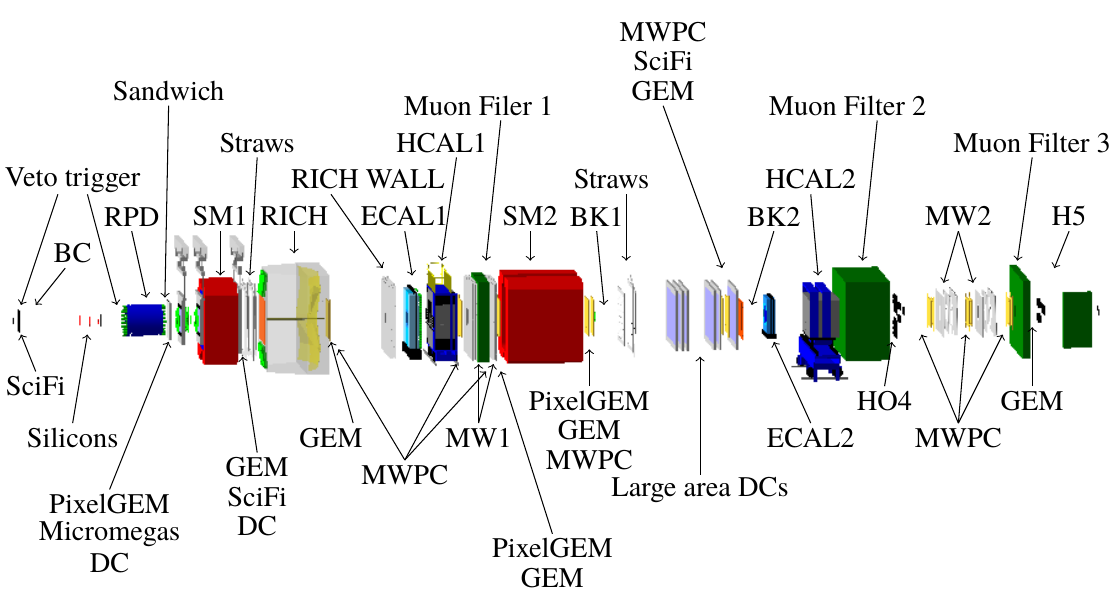
\includegraphics[width=\textwidth]{detector_layout}
	\caption{The layout of COMPASS detectors. The length of whole setup is around 50 meters. Pion beam comes from the left side of detectors and hits the target, which is surrounded by recoil-proton detector (RPD). On the right side of target, two different sets of detectors are used to measure out-going particles with small and large scattering angles.}
	\label{fig:detec_layout}	
\end{figure*}

\subsection{Particle beam and target}
To create the projectile particle beam, the proton beam, which is accelerated by the Super Proton Synchrotron (SPS), is firstly directed into Beryllium. From the nuclear reaction between proton and Beryllium nucleus, a secondary hadron particle beam is created, which functions as incoming particle beam for the scattering experiment. In this project, the hadron beam is selected to be negative charged pion beam. But a small fraction of Kaon (\SI{2.4}{\percent}) can also exist in the incoming particle beam. The proton target, onto which pion beam is diverted, is in form of liquid hydrogen stored in a \SI{40}{\centi\meter} height cylindrical container. 

\subsection{Detector layout}
\label{subsec:Detector_layout}
\begin{figure}[!th]
	\centering
	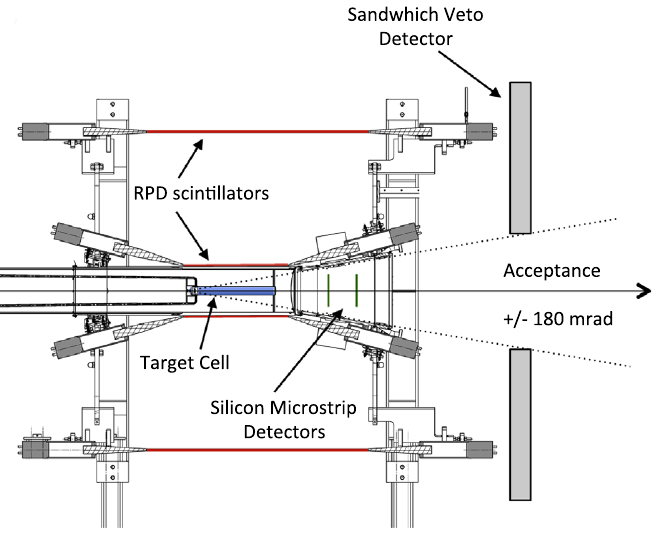
\includegraphics[width=0.5\textwidth]{sandwich}
	\caption{Scheme of detectors around the target region. The sandwich veto on the right prevent unmeasurable events with large scattering angles. Source: \cite{sandwich}}
	\label{fig:sandwich}
\end{figure}

The layout of COMPASS detectors is shown in figure \ref{fig:detec_layout}. Proton target is located inside the RPD (recoil-proton detector). On the left of target locate SciFi (scintillating fiber), BC (Beam counter) and silicon detectors. The coincidence of signals from SciFi and BC is used for the beam trigger, setting the time reference of whole system. The silicon detectors are applied for determining the location of projectile beam, which is further used to calculate the position of primary vertex. On the downstream very close to the target, there are sandwich veto and PixelGEM/Micromegas/DC (Pixel GEM detector, micromegas detectors and drift chamber). The function of sandwich veto is to reject the signal readout when the scattering polar angle of out-going particle is too large to measure. The structure of sandwich veto can be seen in figure \ref{fig:sandwich}, where the veto can be triggered if polar angle is out of acceptance range. Behind the sandwich veto, PixelGEM/Micromegas/DC detectors are implemented to measure the angles of out-going particles with high accuracy and resolution. On the downstream further away from the target, two different sets of detectors are set up for measuring out-going particles with small and large scattering angles. 

The first set, located in the front, is used as large angle spectrometer (LAS). The major components of LAS are SM1 (solenoid magnet 1), tracking detectors, RICH (ring-image Cherenkov detector), ECAL1, HCAL1 and Muon filter. SM1 provides the magnetic field to deviate charged particles. The degree of deviation is measured by the tracking detectors on the both sides, which can calculate the momentum of out-going charged particles. The RICH detector on the right side on SM1 is used to improve the permanence of experiment by separating $\pi$ and $K$ in high intensity environment\cite{RICH}. ECAL1 is an electromagnetic calorimeter used to measure the energy of particles like electrons or photons while HCAL1, a hadron calorimeter, is used to measure the energy of hadron particles. Muon can be identified by tracking detectors behind a muon filter, which intercepts every particles except muon.

The second set, located at the end of downstream, is deployed as small angle spectrometer (SAS). Most of its components have the same functionalities as their counterparts in LAS. The main additional detectors in SAS contains two BKs (beam killer), which are basically two scintillating counters. They are used to veto the non-interacting particle beams\cite{sandwich}.







\section{Data and interaction}
The data recorded by multiple detectors are stored in different partitions. Before carrying out the stability test in this project, the data being analyzed are already pre-selected. In this section, an overview about data storage and pre-selection is discussed, followed by a short introduction of probable interaction giving rise to selected data.

\begin{figure}[t!]
	\centering
	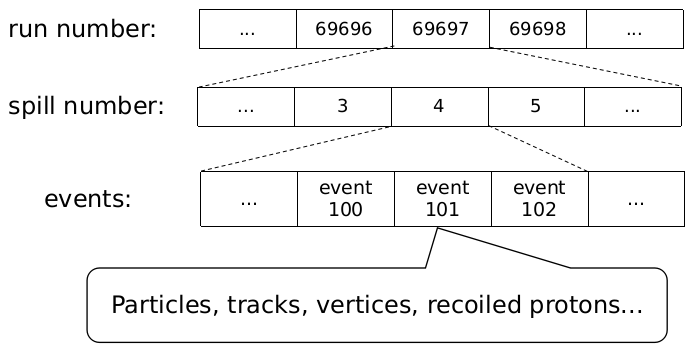
\includegraphics[width=0.5\textwidth]{data_storage}
	\caption{Scheme of data storage structure. Data from the detectors are categorized into three different levels.}
	\label{fig:data_storage}
\end{figure}

\subsection{Data storage}
There are three different partition levels regarding the data storage, as is shown in picture \ref{fig:data_storage}. First, the whole data are stored with different run number. The event data with same run number are further divided into different spill number. One spill corresponds to one period of process, in which the particle beam is bunched and de-bunched. Time expansion of each spill is around 48 seconds \cite{COMPASS}, which is time period of SPS (super proton synchrotron). Similarly, each spill contains large amount of events. One event represents a single scattering between $\pi$ and proton and it contains all data of the corresponding event from detectors such as tracking detectors or calorimeters.

\subsection{Data preselection}
\label{subsec:data_preselection}
The data used in this stability test are not raw data coming directly from detectors, but rather being preselected previously. Event is only selected if it meets following 4 conditions: 
\begin{itemize}
	\item A best primary vertex was found
	\item Primary vertex Z-position $Z_{pv}$: $\SI{-200}{\centi\meter} < Z_{pv} < \SI{160}{\centi\meter}$
	\item Exactly one or three charged tracks, leaving the primary vertex
	\item Charge sum of all three tracks $= -1$
\end{itemize}
The first condition requires the existence of primary vertex. This is because the vertex position is not the value that can be directly measured by detectors. It is rather reconstructed by identifying the intersecting point between two charged particle tracks. Thus, there could be no primary vertex constructed in some events, which should be selected out. Second condition excludes the events where outgoing particles are not coming from the interaction on proton target but rather on some detectors. Therefore, the position of primary vertex must be around the target region. The third and fourth condition guarantees the data after selection correspond to the elastic scattering or the interaction where one $\pi$ is scattered into three charged $\pi$.

\subsection{Scattering process}
\label{subsec:photon}
\begin{figure}[thb]
	\centering
	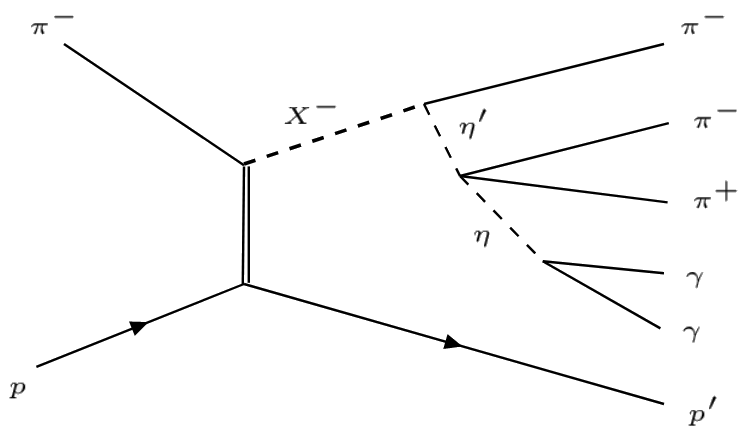
\includegraphics[width=0.5\textwidth]{feymann_diag}
	\caption{Scheme of one possible inelastic scattering between $\pi$ and proton. In such case, $pi^-$ is excited and consecutively decays into 3 charged $\pi$, during which multiple photons can also be emitted.}
	\label{fig:feymann_diag}
\end{figure}

The interaction that is looked into for this stability test is inelastic scattering of one $\pi^-$ scattered into three charged $\pi$. Due to the preselection, charged ejectile particles are very likely to be $\pi^-$, $\pi^+$, $\pi^-$.  One possibility of the interaction is shown in figure \ref{fig:feymann_diag}. By scattering off the proton target, $\pi^-$ is excited into a high energy state ($X$), which in a very short time, decays into $\pi^-$ and $\eta'$. Due to instability of $\eta'$, it finally decays into $\pi^-$ and $\pi^+$ as well. Meanwhile, certain number of photons can also be emitted by electromagnetic radiation. 
\section{Characteristic parameters}
The main method of stability testing is to check the values of multiple parameters in different runs and identify the outliners. In this project, relating parameters are extracted by a data analysis framework called PHAST (Physics Analysis Software Tools). It provides the access to reconstructed events information and tools of data processing.

\begin{figure*}[!ht]
	\centering
	\begin{subfigure}[b]{0.49\textwidth}
		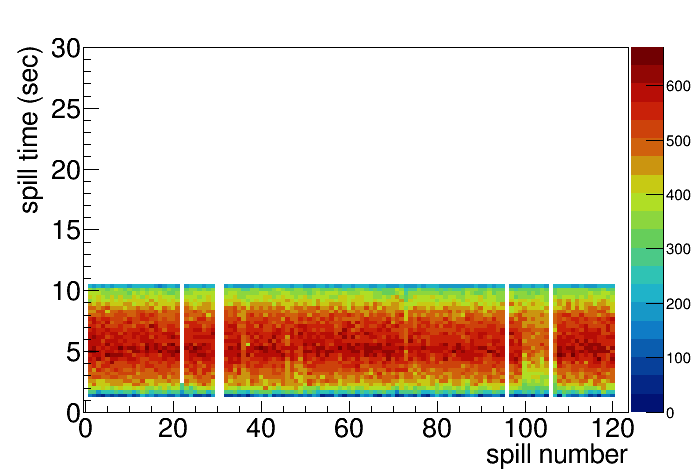
\includegraphics[width=\textwidth]{event_spill_70171}
		\caption{Run 70171}
		\label{fig:EveN_spill_normal}
	\end{subfigure}
	~ %add desired spacing between images, e. g. ~, \quad, \qquad, \hfill etc. 
	%(or a blank line to force the subfigure onto a new line)
	\begin{subfigure}[b]{0.49\textwidth}
		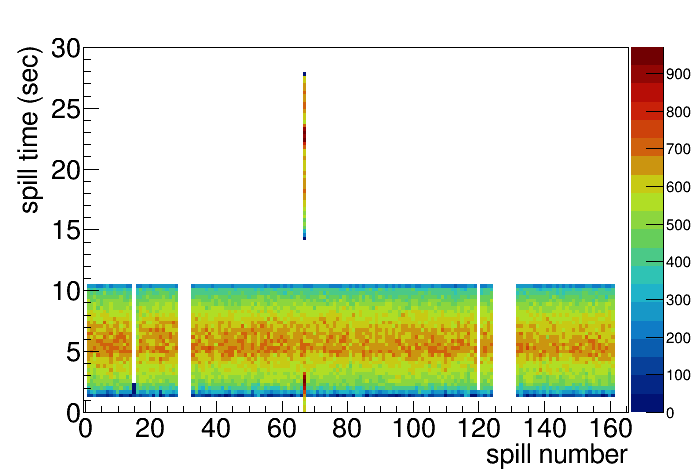
\includegraphics[width=\textwidth]{strange_spill_70195}
		\caption{Run 70195}
		\label{fig:EveN_spill_abnormal}
	\end{subfigure}
	\caption{Temporal distribution of event numbers for each spill number. The color band represents the number of events per 0.3 seconds (time resolution) for each spill. The y axes represent the time from starting moment of each spill. (a) A normal temporal distribution (run number = 70171). The effective time expansion of particle beam is around 9s and distribution of each spill is centrally concentrated. (b) An abnormal temporal distribution (run number = 70195). Particle beam occurred in inactive time period.}
	\label{fig:animals}
\end{figure*}

\begin{figure*}[!h]
	\centering
	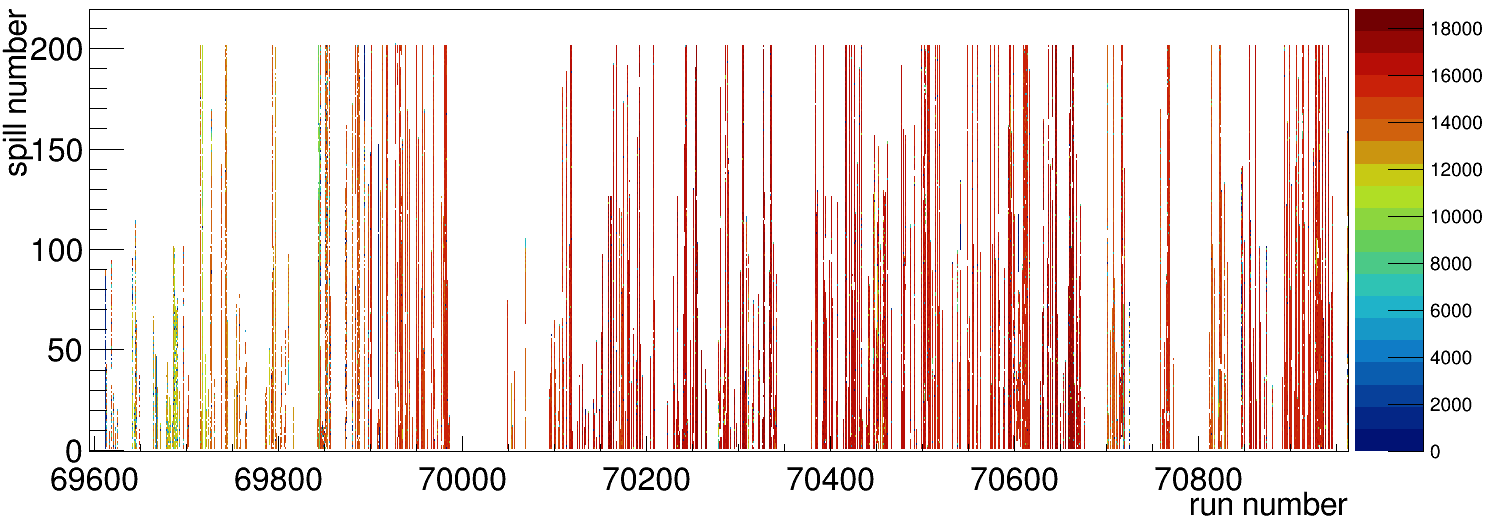
\includegraphics[width=\textwidth]{event_distribution_all}
	\caption{Event distribution with respect to spill number of each run number. The color band shows the number of events in a certain spill of a certain run. The run number ranges from $69595 \sim 70963$ while spill number of each run ranges from 0 to 200. The number of events per spill can goes up to 18000 whereas it could also amount to only few thousands or less, especially in the beginning of experiment. }
	\label{fig:event_distribution_all}
\end{figure*}

\subsection{Number of events}
The number of events for each run can be vastly different after the preselection. By using PHAST data analysis framework, the number of events for each spill of every run is counted and plotted. Since the beam only exist in certain time interval of spill, event numbers are not spread uniformly throughout the whole period of spill. From figure \ref{fig:EveN_spill_normal}, one can easily see that, in normal cases, events are only distributed on the time interval \SI{1.2}{\second} $\sim$ \SI{10.5}{\second} of the spill period. There is a short dead period of \SI{1.2}{\second} before the start of particle beam and a long inactive period after \SI{10.5}{\second} till the end of spill (at around \SI{48}{\second}). However, as is shown in figure \ref{fig:EveN_spill_abnormal}, there exists one abnormal run, where the effective time interval of one spill is more than 2 times larger than the normal one. To be exact, the particle beam occurs not only during the inactive time interval right at the beginning of spill (\SI{0}{\second} $\sim$ \SI{1.2}{\second}), but also after the first stop of beam (\SI{14.1}{\second} $\sim$ \SI{27.9}{\second}). Such abnormality could probably result from a trigger problem, due to which events are recorded with wrong time scale\footnote[2]{The abnormal run 70195 is ruled out for the following analysis}.

After selecting out the run with abnormal temporal distribution discussed above, the number of events can be compared for each spill in every run, as is shown in figure \ref{fig:event_distribution_all}. The event number distribution is quite uneven throughout the experiment after the preselection. Runs in the beginning usually have low values of event counting and most of them don't have any event in some spills. Moreover, there even exist large number of vacant runs with no events in all spills. Therefore, one can consider the number of events of each run as the characteristic parameter to test the stability of the experiment. However, analyses such as invariant mass of three pion mass are independent from the number of events one has for each run. Thus, the variation of event distribution throughout the experiment could have little or no effect towards results of the analyses.
\begin{figure}[!b]
	\centering
	\begin{subfigure}[t]{0.5\textwidth}
		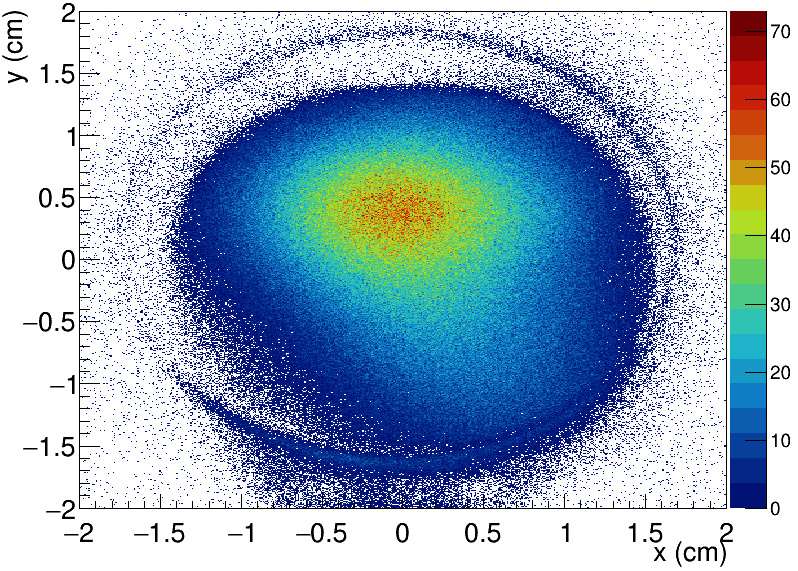
\includegraphics[width=\textwidth]{Prim_vertex_70171}
		\caption{Primary vertex}
		\label{fig:Prim_vertex_70171}
	\end{subfigure}
	~ %add desired spacing between images, e. g. ~, \quad, \qquad, \hfill etc. 
	%(or a blank line to force the subfigure onto a new line)
	\begin{subfigure}[b]{0.5\textwidth}
		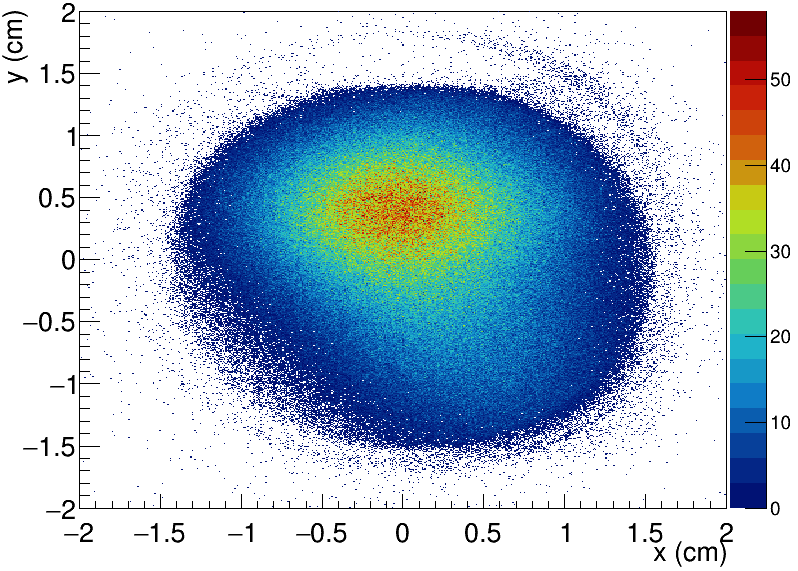
\includegraphics[width=\textwidth]{sec_vertex_70171}
		\caption{Primary vertex with three outgoing particles}
		\label{fig:sec_vertex_70171}
	\end{subfigure}
	\caption{vertex position distribution in x-y plane (vertical plane to z direction of the particle beam). The color band represents the number of vertices in corresponding location. Spacial resolution of x and y are both \SI{0.008}{\centi\meter}. (a) Distribution of primary vertices, in which a strange halo structure appears in the graph. (b) Distribution of primary vertices with three outgoing particles, where the halo disappears.}
	\label{fig:ver_pos}
\end{figure}
\subsection{Vertex positions}
The next parameter that could be investigated is the position of vertices. The location of vertices cannot be measured directly from the detectors but rather reconstructed by the charged particle tracks. There are only two types of vertice of each event extracted from PHAST: primary vertices and non-primary vertices. Generally, the vertex position is determined by finding the intercept point between two reconstructed tracks. If this intercept point also lies on the track of the incoming particle, it is considered to be a primary vertex. If not, it is considered to be a non-primary vertex. 


As discussed in subsection \ref{subsec:data_preselection}, events which survived the  preselection contain either one charged track or three charged tracks. Events containing one charged track correspond to elastic scattering while event with three charged tracks correspond to inelastic scattering. In case of elastic scattering, since there is only one out-going particle track and one incoming particle track, all vertices being reconstructed are primary vertices. On the other hand, non-primary vertices could only exists in inelastic scattering. This can be better explained by looking at the vertices position map shown in figure \ref{fig:ver_pos}. The first graph, figure \ref{fig:Prim_vertex_70171}, shows the primary vertex position. As one can easily see, most of the vertex positions are on the liquid hydrogen target, which is located at around $\SI{-1.4}{\centi\meter} \sim \SI{1.5}{\centi\meter}$ in x direction and $\SI{-1.5}{\centi\meter} \sim \SI{1.3}{\centi\meter}$ in y direction. Additional, there is halo shaped data points surrounding target. The cause behind this strange shape is elastic scattering between the $\pi$ beam and container of liquid hydrogen. From the vertices distribution on the center, one can see that the particle density of the beam is roughly Gaussian distributed in the cross section. In other words, there are more incoming particles in the central area of the beam than the peripheral area, leading to the decreasing of vertex density in the outward direction. But when the beam hits the metallic container, the vertex density surges due to the increase of elastic scattering of the beam $\pi^-$ and the container. Therefore, the vertices on the halo are most likely to be primary vertices with one $\pi^-$ going out. This can be further proved by checking the position of primary vertices with three outgoing particles. In figure \ref{fig:sec_vertex_70171}, the strange halo structure disappears, which indicates that most of events with three out-going particles corresponds to the inelastic scattering between the pion beam and hydrogen target.  
\begin{figure*}[!ht]
	\centering
	\vspace{1cm}
	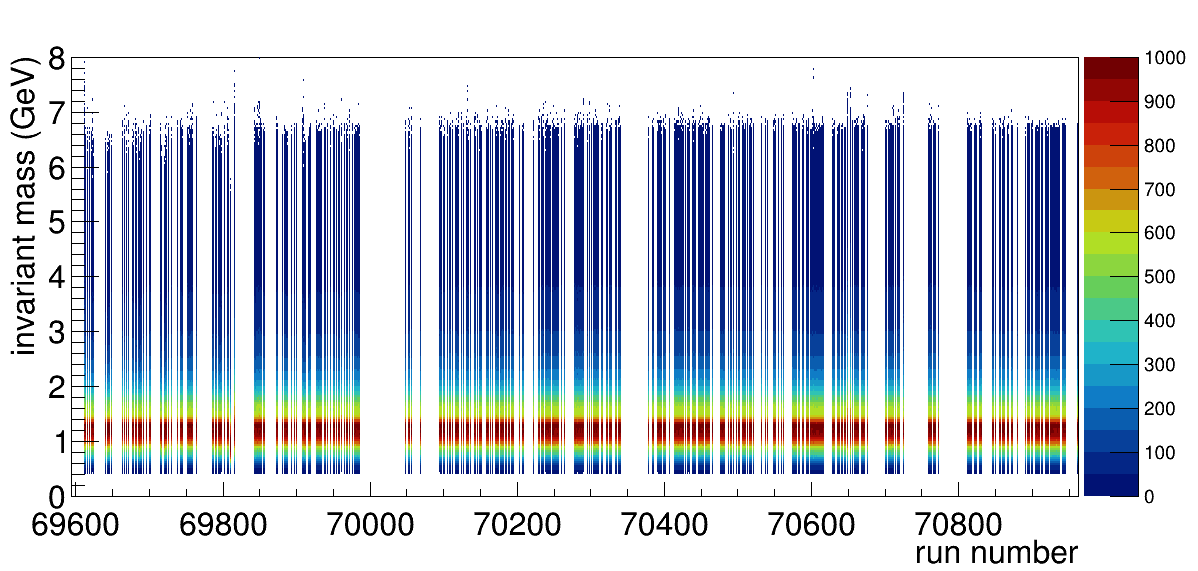
\includegraphics[width=\textwidth]{Three_pion_mass_his}
	\caption{Histogram of the three pion invariant mass for each run. The colors inside the histogram represent the number of events for each run and invariant mass. To better compare and conceive the structure of the distribution between runs visually, the maximal value of each distribution is normalized to 1000. As one can easily notice that maximal value or peak of distribution locates around \SI{1.3}{\giga\electronvolt} for almost every run.}
	\label{fig:Three_pion_mass_his}
	\vspace{2 cm}
	
	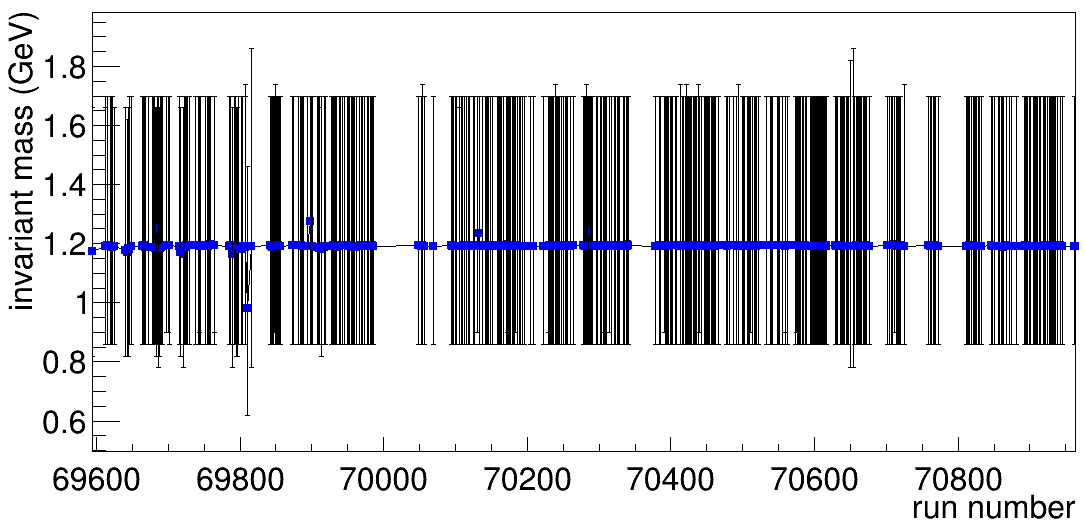
\includegraphics[width=\textwidth]{Three_pion_mass_Graph}
	\caption{Comparison of primary peak position and half maximum range from each run. The blue dots shows the value of fitting parameter $a_1$, which correspond to positions of primary peak. The error bar the range of half maximum. An abnormal run 69811 (denoted in red circle) can be easily spotted in this plot.}
	\label{fig:Three_pion_mass_Graph}
	\vspace{3cm}
\end{figure*}
\subsection{Three pions invaraint mass}
\begin{figure*}[t!]
	\centering
	\begin{subfigure}{0.48\textwidth}
		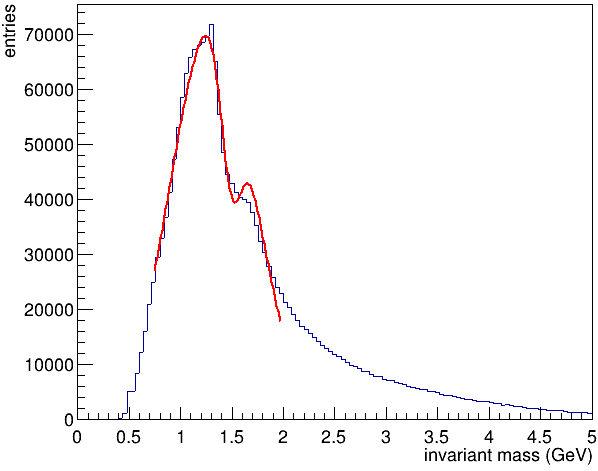
\includegraphics[width=\textwidth]{Three_pion_mass_fitting}
		\caption{run 70171}
		\label{fig:Three_pion_mass_fitting}
	\end{subfigure}
	\begin{subfigure}{0.48\textwidth}
		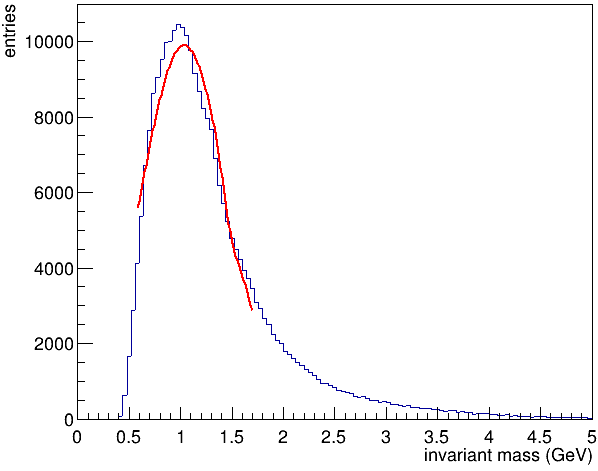
\includegraphics[width=\textwidth]{Three_pion_mass_69811}
		\caption{run 69811}
		\label{fig:Three_pion_mass_69811}
	\end{subfigure}
	\caption{Three pion invariant mass distribution and their corresponding fit result. The fit range corresponds to \SI{30}{\percent} of of maximal value of the distribution. (a) Distribution of a normal run. The first peak (primary) locates at around \SI{1.3}{\giga\electronvolt}. The red curve matches data well  around the primary peak, but poorly around the second peak. (b) Distribution of an abnormal run. No second peak can be found on the right side of primary peak. Parameter $a_1$ is fitted to be \SI{1.034}{\giga\electronvolt}, which is slightly larger than a usual value due to the bad fit. }
	\label{fig:pion_mass}
\end{figure*}
The most obvious parameter that can be used for stability test should be the invariant mass distribution of three out-going pions, as is shown in figure \ref{fig:Three_pion_mass_his}. Since the total number of events in each run is significantly different, the invariant mass distribution is normalized so that the maximum value of the distribution is always equal to 1000. By such normalization, one can easily notice that the maximal value locates at the same place for each run. Looking at the $3\pi$ spectrum of a single run (figure \ref{fig:Three_pion_mass_fitting}), one can see a double peak structure. The first peak is located around \SI{1.3}{\giga\electronvolt}, which is followed by a small second peak around \SI{1.67}{\giga\electronvolt} on the right side. To test the stability of this throughout all analysis, the position of the first peak is determined by fitting the histogram with following function:
\begin{equation}
f(x) = a_0 \cdot \Big(\mathcal{N}(a_1, a_2^2)+a_3 \cdot \mathcal{N}(a_4, a_5^2)\Big)
\end{equation}
where $\mathcal{N}(\mu,\sigma^2)$ represents a Gaussian distribution with mean value $\mu$ and standard deviation $\sigma$. $a_0$, $a_1$, $a_2$, $a_3$, $a_4$ and $a_5$ are six fitting parameters with initial values: $a_0 \sim$ maximal value, $a_1 \sim 1$, $a_2 \sim 1$, $a_3 \sim 0.01$ and $a_5 \sim 1$. Through trail and errors, $a_4$ is fixed to be 1.49 to optimize the fitting curve for the first peak.

The fitting result of a typical distribution is shown as the red curve in figure \ref{fig:Three_pion_mass_fitting}. The position of the primary peak is related to the value of $a_1$, fitted to be \SI{1.305}{\giga\electronvolt}. Figure \ref{fig:Three_pion_mass_Graph} shows the result after carrying out such a fit for each run and calculating the position of primary peak as well as the full width at half maximum of corresponding distribution. One outliner, run number 69811, can easily be identified (the red circle in figure \ref{fig:Three_pion_mass_Graph}). Figure \ref{fig:Three_pion_mass_69811} shows its corresponding distribution. It is not hard to discover that there exists no noticeable second peak while its primary peak shifts a little to smaller values, which mirrors in the low value shown in figure \ref{fig:Three_pion_mass_Graph}.
\subsection{Total invariant mass}
The next parameter worth investigating is the invariant mass of all out-going particles, i.e. out-going pions and photons. The four-momentum of pions can be obtained in the same way as seen in the previous subsection. To obtain the four-momentum of the photons, energy cuts are applied differently to the data coming from two electromagnetic calorimeters (ECAL) and remaining photons are all assumed to come from primary vertex.
\subsubsection{Photon energy cut}
\begin{figure}[!t]
	\centering
	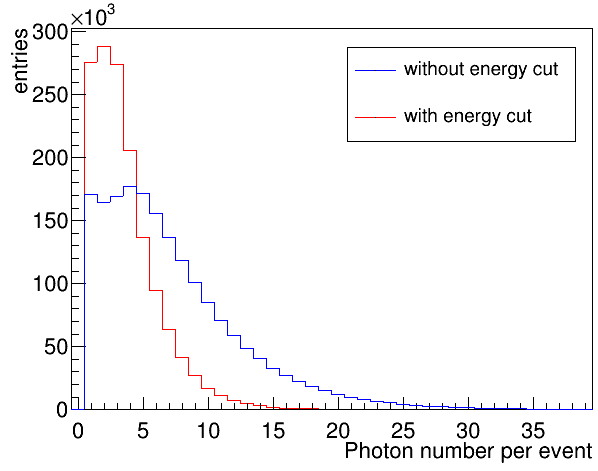
\includegraphics[width=0.5\textwidth]{photon_energy_cut}
	\caption{Effect of energy cut of photons. On the x axis is the number of photons reconstructed in both ECALs and on the y axis, amount of number of events (entries) which contain the corresponding photons are shown. Blue line is the histogram of events without photon energy cut and red line events with photon energy cut. As can be seen easily that number of events with small number of photons are increased significantly after energy cut.}
	\label{fig:photon_energy_cut}
\end{figure}
As discussed in subsection \ref{subsec:photon}, photons can also be emitted during the interaction. In contrast to the charged pions, which leave tracks in tracking detectors via ionization, photons have no charge and, therefore, no track can be found. The only way to identify photons is by its energy deposits in ECAL. However, ECAL can only gives the energy of each reconstructed photon and the direction of its momentum cannot be determined by any detectors in COMPASS experiment. Thus, the vertex which photon comes from cannot be determined neither. On the other hand, photons reconstructed in ECALs could also come from the background instead of scattering vertex. Photons from background are mainly generated by bremsstrahlung between beam particles or outgoing pions and the material of detectors. Nevertheless, those background photons usually have a very small energy compared to those coming out of scattering vertices. Thus, to differentiate the photons from scattering vertices and photons from background, energy cuts are applied to the reconstructed photons of each calorimeter. Considering only photons from the scattering, since the ECAL1 photons have larger scattering angle than ECAL2 photons, energy deposits on the ECAL1 are generally smaller than on the ECAL2. Thus the energy cut for ECAL1 photons should be smaller than the cut for ECAL2 photons, as is shown by following:

\begin{center}
	\begin{tabular}{c||c}
		Calorimeter & Energy cut      \\
		\hline
		ECAL1       & \textgreater{}\SI{1}{\giga\electronvolt} \\
		\hline
		ECAL2       & \textgreater{}\SI{4}{\giga\electronvolt}
	\end{tabular}
\end{center}



Photons with energy smaller than energy cut are selected out on both ECALs. The result of energy cut is shown in figure \ref{fig:photon_energy_cut}. As one can easily notice that, without energy cut, there are sufficient amount of events that could have more than 10 photons in total detected by calorimeters, which is highly unlikely in scattering process. Once energy cuts are applied and photons with low energy being removed, almost all events have only less than 10 photons. In the end, by assuming all photons after energy cuts come from the primary vertex, 4-momentum of each photon can, thus, be obtained.
\subsubsection{Total invariant mass}
\begin{figure}[!t]
	\centering
	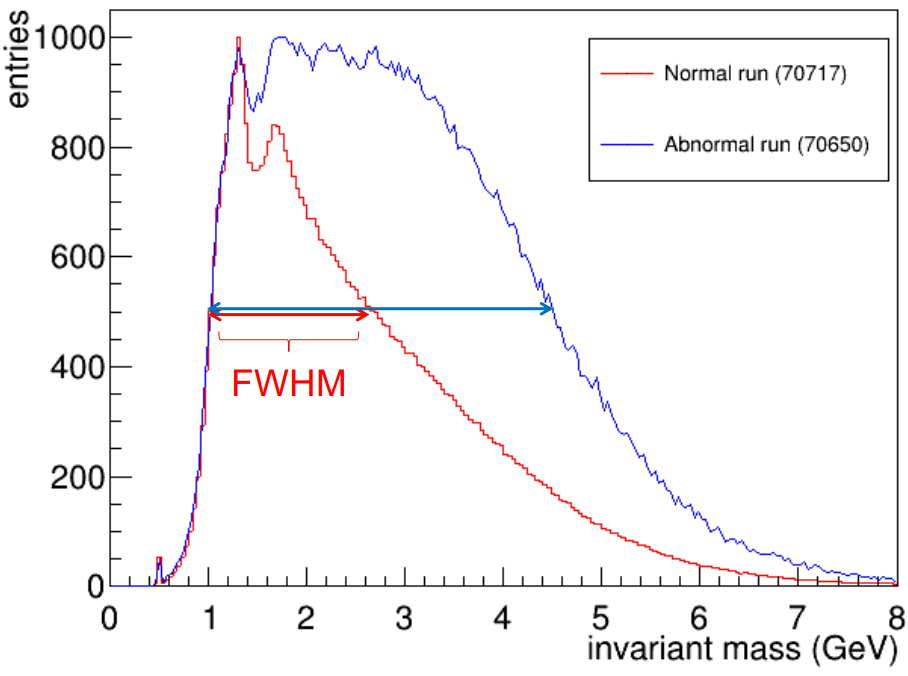
\includegraphics[width=0.5\textwidth]{Total_mass_comp}
	\caption{Comparison of normalized total invariant mass distribution between normal run and abnormal run. Both maximal value of both distribution are set to be 1000. On the x axis shows the value of total invariant mass and on the y axis shows the entries of corresponding value. FWHM is width of the range between two points, which corresponds to 500 value. As can be seen very clearly that the abnormal run (70650) has a much larger FWHM value than the normal run (70717).}
	\label{fig:Total_mass_comp}
\end{figure}
Total invariant mass is a very important parameter, which corresponds to the mass of intermediate unknown resonance state X (in figure \ref{fig:feymann_diag}). Figure \ref{fig:Total_mass_his} shows the normalized invariant mass distribution for each run. For most of runs, a clear peak can be seen between \SI{1}{\giga\electronvolt} to \SI{2}{\giga\electronvolt} while the spectrum falls afterwards. However, there are several runs which have much longer range of high entry value (shown in red boxes). The invariant mass distribution of an normal run (run 70717) is shown in figure \ref{fig:Total_mass_comp} (red line), compared with that from an abnormal runs (run number 70650, blue line). One can immediately see that the abnormal run has a much bigger full width half maximum (FWHM) value than the normal run. Both runs have their first peak at the same position. But for the abnormal run, the number of entries does not go down immediately after second peak. To examine this phenomenon throughout the whole data, the FWHM value is calculated for each run (see figure \ref{fig:Total_mass_FWHM}). For most of runs, the high number of entries concentrate on the range between \SI{1.4}{\giga\electronvolt} and \SI{1.8}{\giga\electronvolt}. But some outliners can have much larger FWHM value up to \SI{3.5}{\giga\electronvolt}. On the other hand, some runs have a slightly smaller value, ranging from \SI{1.3}{\giga\electronvolt} to \SI{1.4}{\giga\electronvolt}.

Two possibilities comes to mind for this abnormal phenomenon. One is related to unexpected variation of initial scattering conditions of interaction process, such as energy of beams. The other is related to the malfunction of calorimeters because the reconstructed photons seems to be the main cause if one compares the abnormality of three pion invariant mass and total invariant mass . The first could be checked directly by the recoil proton ($p'$ in figure \ref{fig:feymann_diag}).

\begin{figure*}[!ht]
	\centering
	\vspace{2cm}
	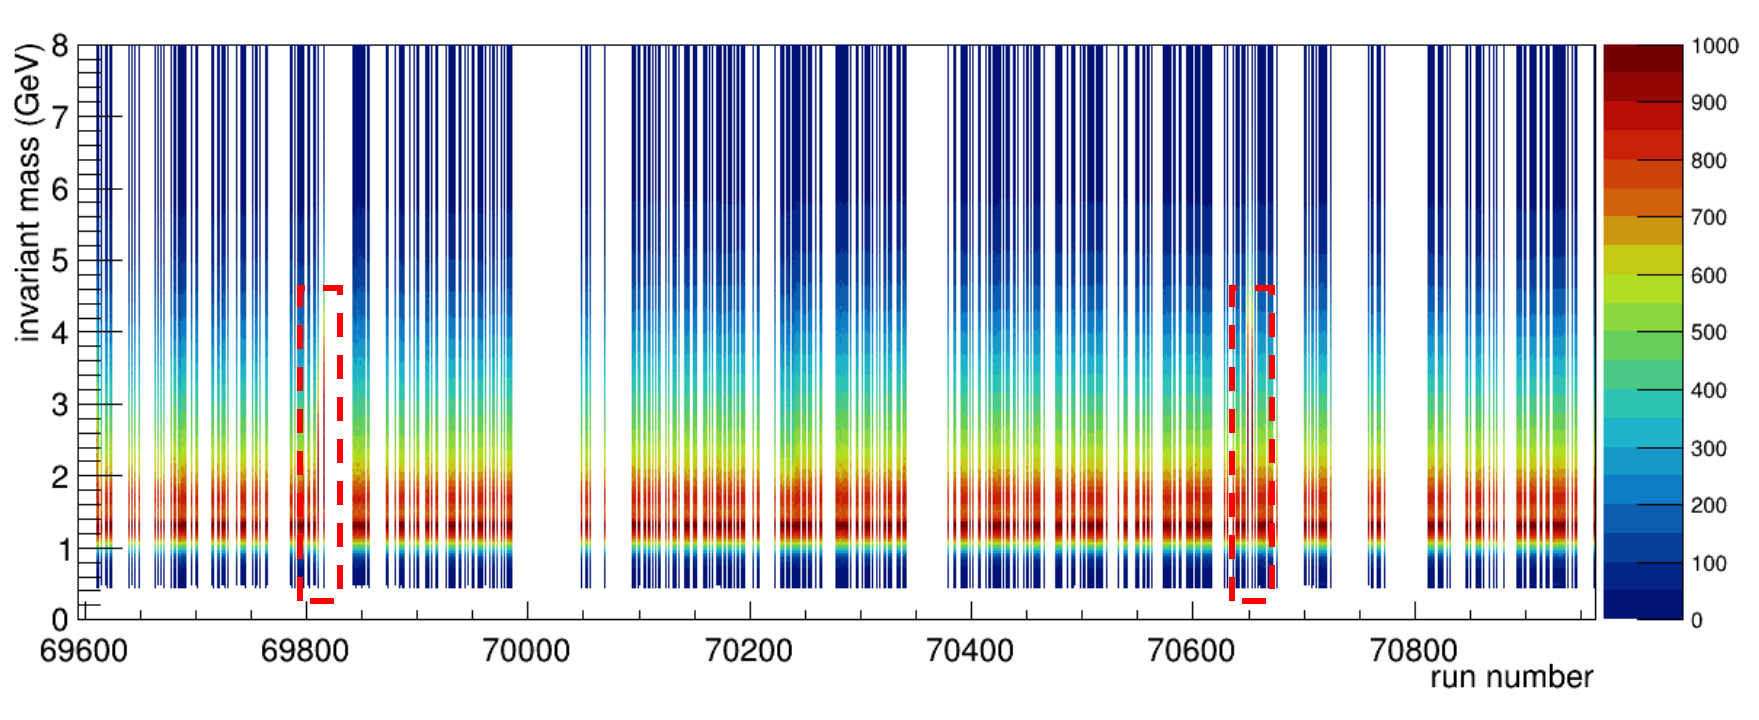
\includegraphics[width=\textwidth]{Total_mass_his}
	\caption{Histogram of the total invariant mass distribution. The colors inside the histogram represent the number of events corresponding to the run number and invariant mass. To see the disparities of each run more clearly, the distribution of invariant mass is normalized with maximum value fixed to be 1000. In the red dashed rectangles, it can be seen that the red strokes are much longer than the normal runs.}
	\label{fig:Total_mass_his}
	\vspace{2 cm}
	
	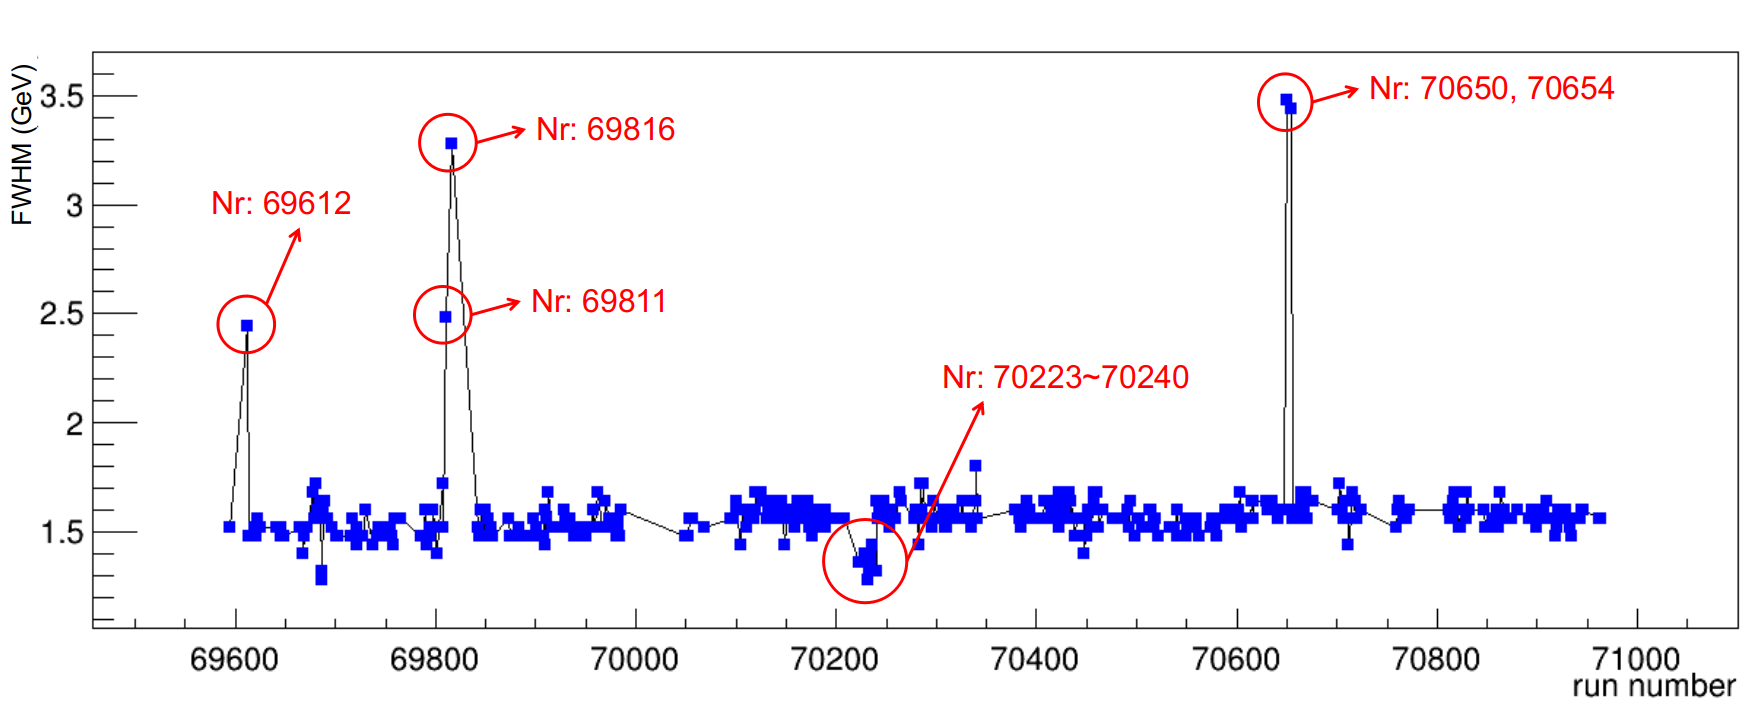
\includegraphics[width=\textwidth]{Total_mass_FWHM}
	\caption{Value of full width at half maximum of the total invariant distribution for each run. The typical value of FWHM for a normal run is around \SI{1.5}{\giga\electronvolt}.There are several outliners that have much bigger FWHM than the usual ones. Also there is a range of runs 70223 $\sim$ 70240 that have a slightly smaller value of FWHM value. }
	\label{fig:Total_mass_FWHM}
	\vspace{3cm}
\end{figure*}

\subsection{Recoil proton}

\label{subsec:recoil_proton}
As discussed in subsection \ref{subsec:Detector_layout} and depicted in figure \ref{fig:sandwich}, the recoil-proton detector has a cylindrical shape, surrounding the liquid hydrogen target. Any proton knocked out of the target would be directly detected by RPD. RPD contains two layers: inner layer and outer layer. Both layers can measure the time and location of recoil proton passing through. Energy or velocity of the recoil proton can be obtained by calculating time difference of two layers. However, to calculated the scattering angle of recoil proton (or recoil angle), except the locations measured by two layers of RPD, one must also know the position of primary vertex in the corresponding event. Angular distribution of recoil proton is shown in figure \ref{fig:Recoil_proton_comp}. For both runs, the distributions peak at around $\theta=\SI{1.35}{\radian} = 77.35^{\circ}$, where $\theta$ is angle between the z axis and the momentum direction of the out-going proton. The disparities between the normal run and the abnormal run are shown in the lower half of the distribution. For the abnormal run, a huge bump occurs on the left side of the peak below \SI{45}{\percent} of the maximum value, which can be reflected numerically by calculating the width of a certain height, such as \SI{23}{\percent} of the maximum value.

\begin{figure}[!b]
	\centering
	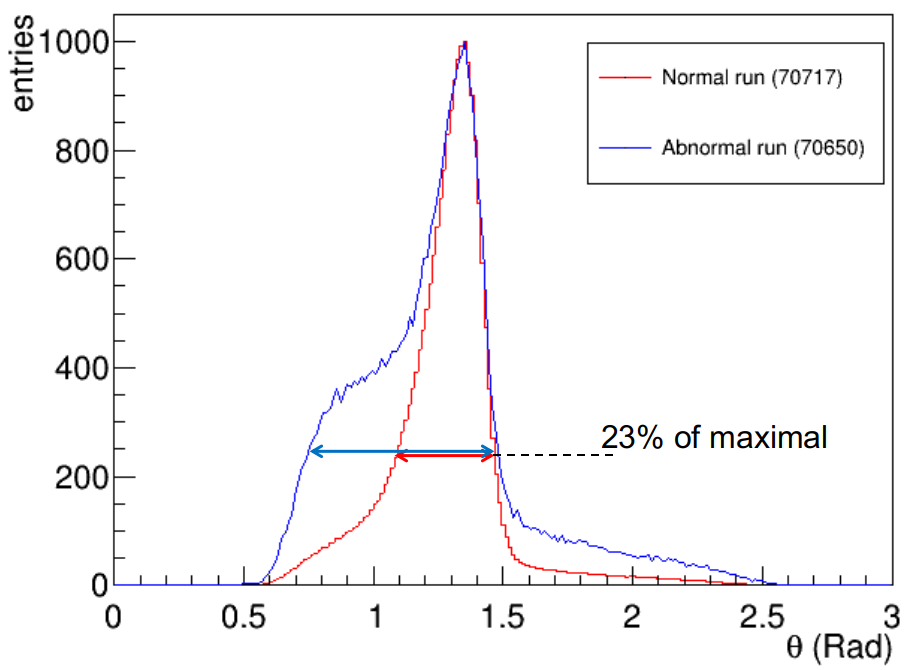
\includegraphics[width=0.5\textwidth]{Recoil_proton_comp}
	\caption{Normalized angular distribution of the recoil proton. On the x axis is the recoil angle $\theta$ of out-going proton with respect to z axis. on the y axis the number of events with the corresponding recoil angle is shown. Red curve represents of a normal distribution from run 70717 and the blue curve is an abnormal distribution from run 70650. Both are normalized so that the maximum value is 1000. }
	\label{fig:Recoil_proton_comp}
\end{figure}

\begin{figure}[!b]
	\centering
	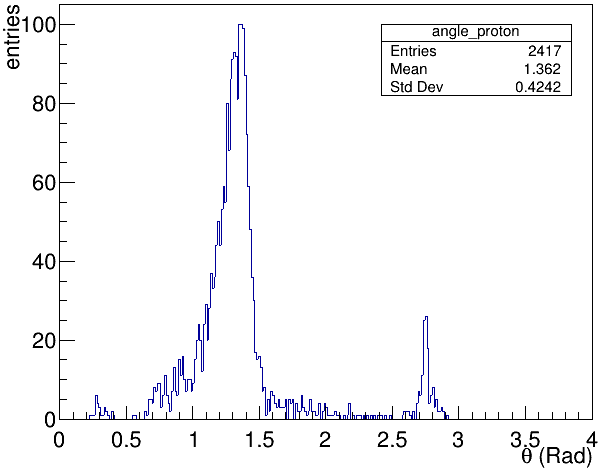
\includegraphics[width=0.5\textwidth]{Recoil_proton_double_peak}
	\caption{Angular distribution of the recoil proton (70054). On the right side of the primary peak another small peak occurs, which corresponds to recoil protons which recoil nearly in the opposite direction of the incoming pion beam. }
	\label{fig:Recoil_proton_double_peak}
\end{figure}

\begin{figure*}[!h]
	\centering
	\vspace{1cm}
	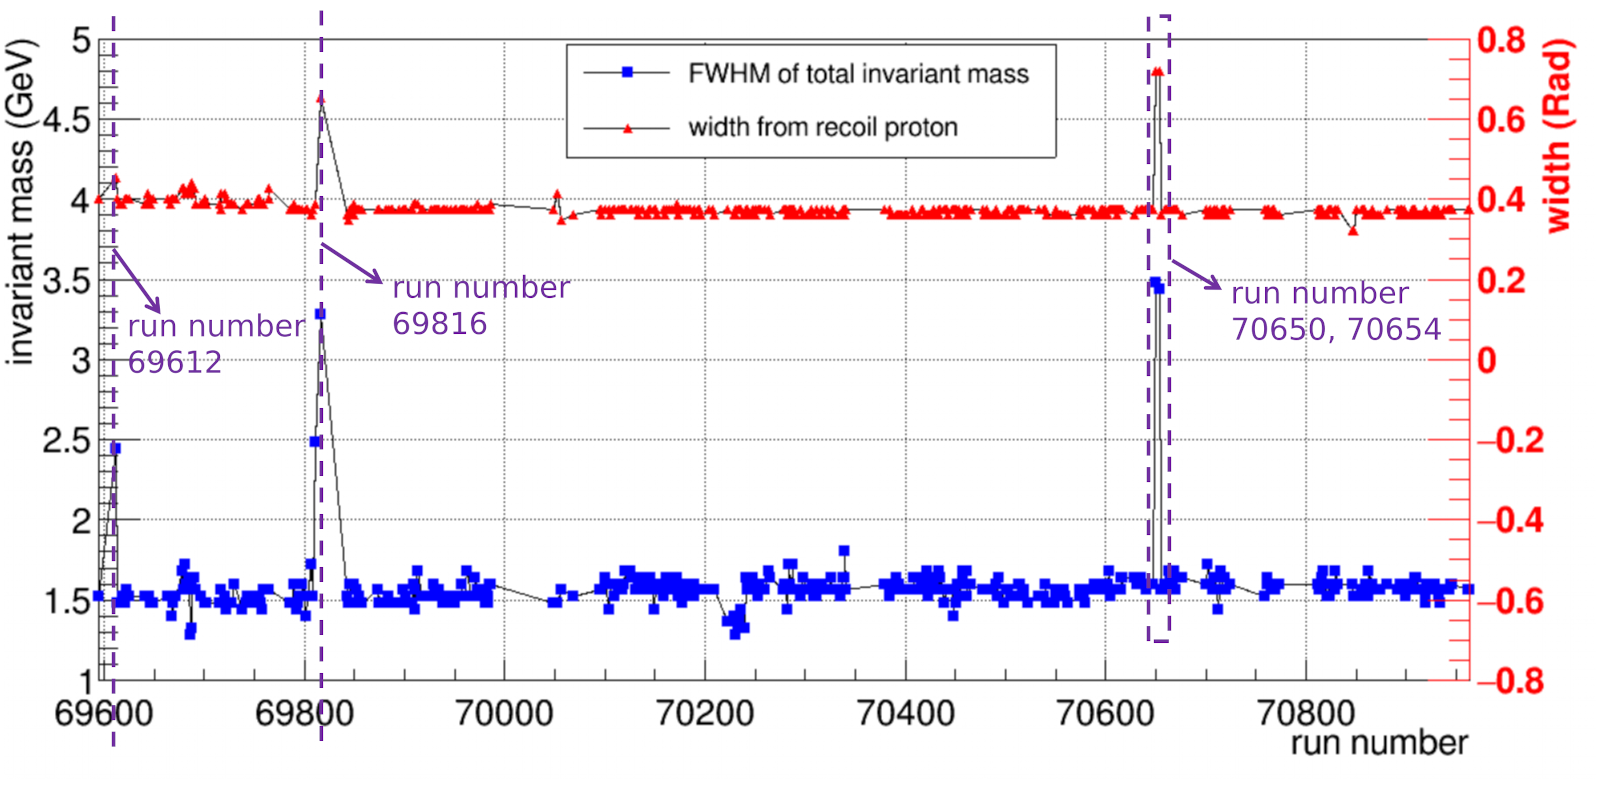
\includegraphics[width=\textwidth]{Total_mass_recoil_proton}
	\caption{Comparison between the FWHM value of total invariant mass (blue) and the width (at 23\% of maximal value) of angular distribution of recoil proton (red). On the right vertical axis are the values of recoil proton width and on the left are the values of invariant mass. Three regions can be found for the evidence of correlation: 69612, 69816 and 70650$\sim$70654. All the abnormal runs are positively correlated between these two parameters.}
	\label{fig:Total_mass_recoil_proton}
	\vspace{1 cm}
	
	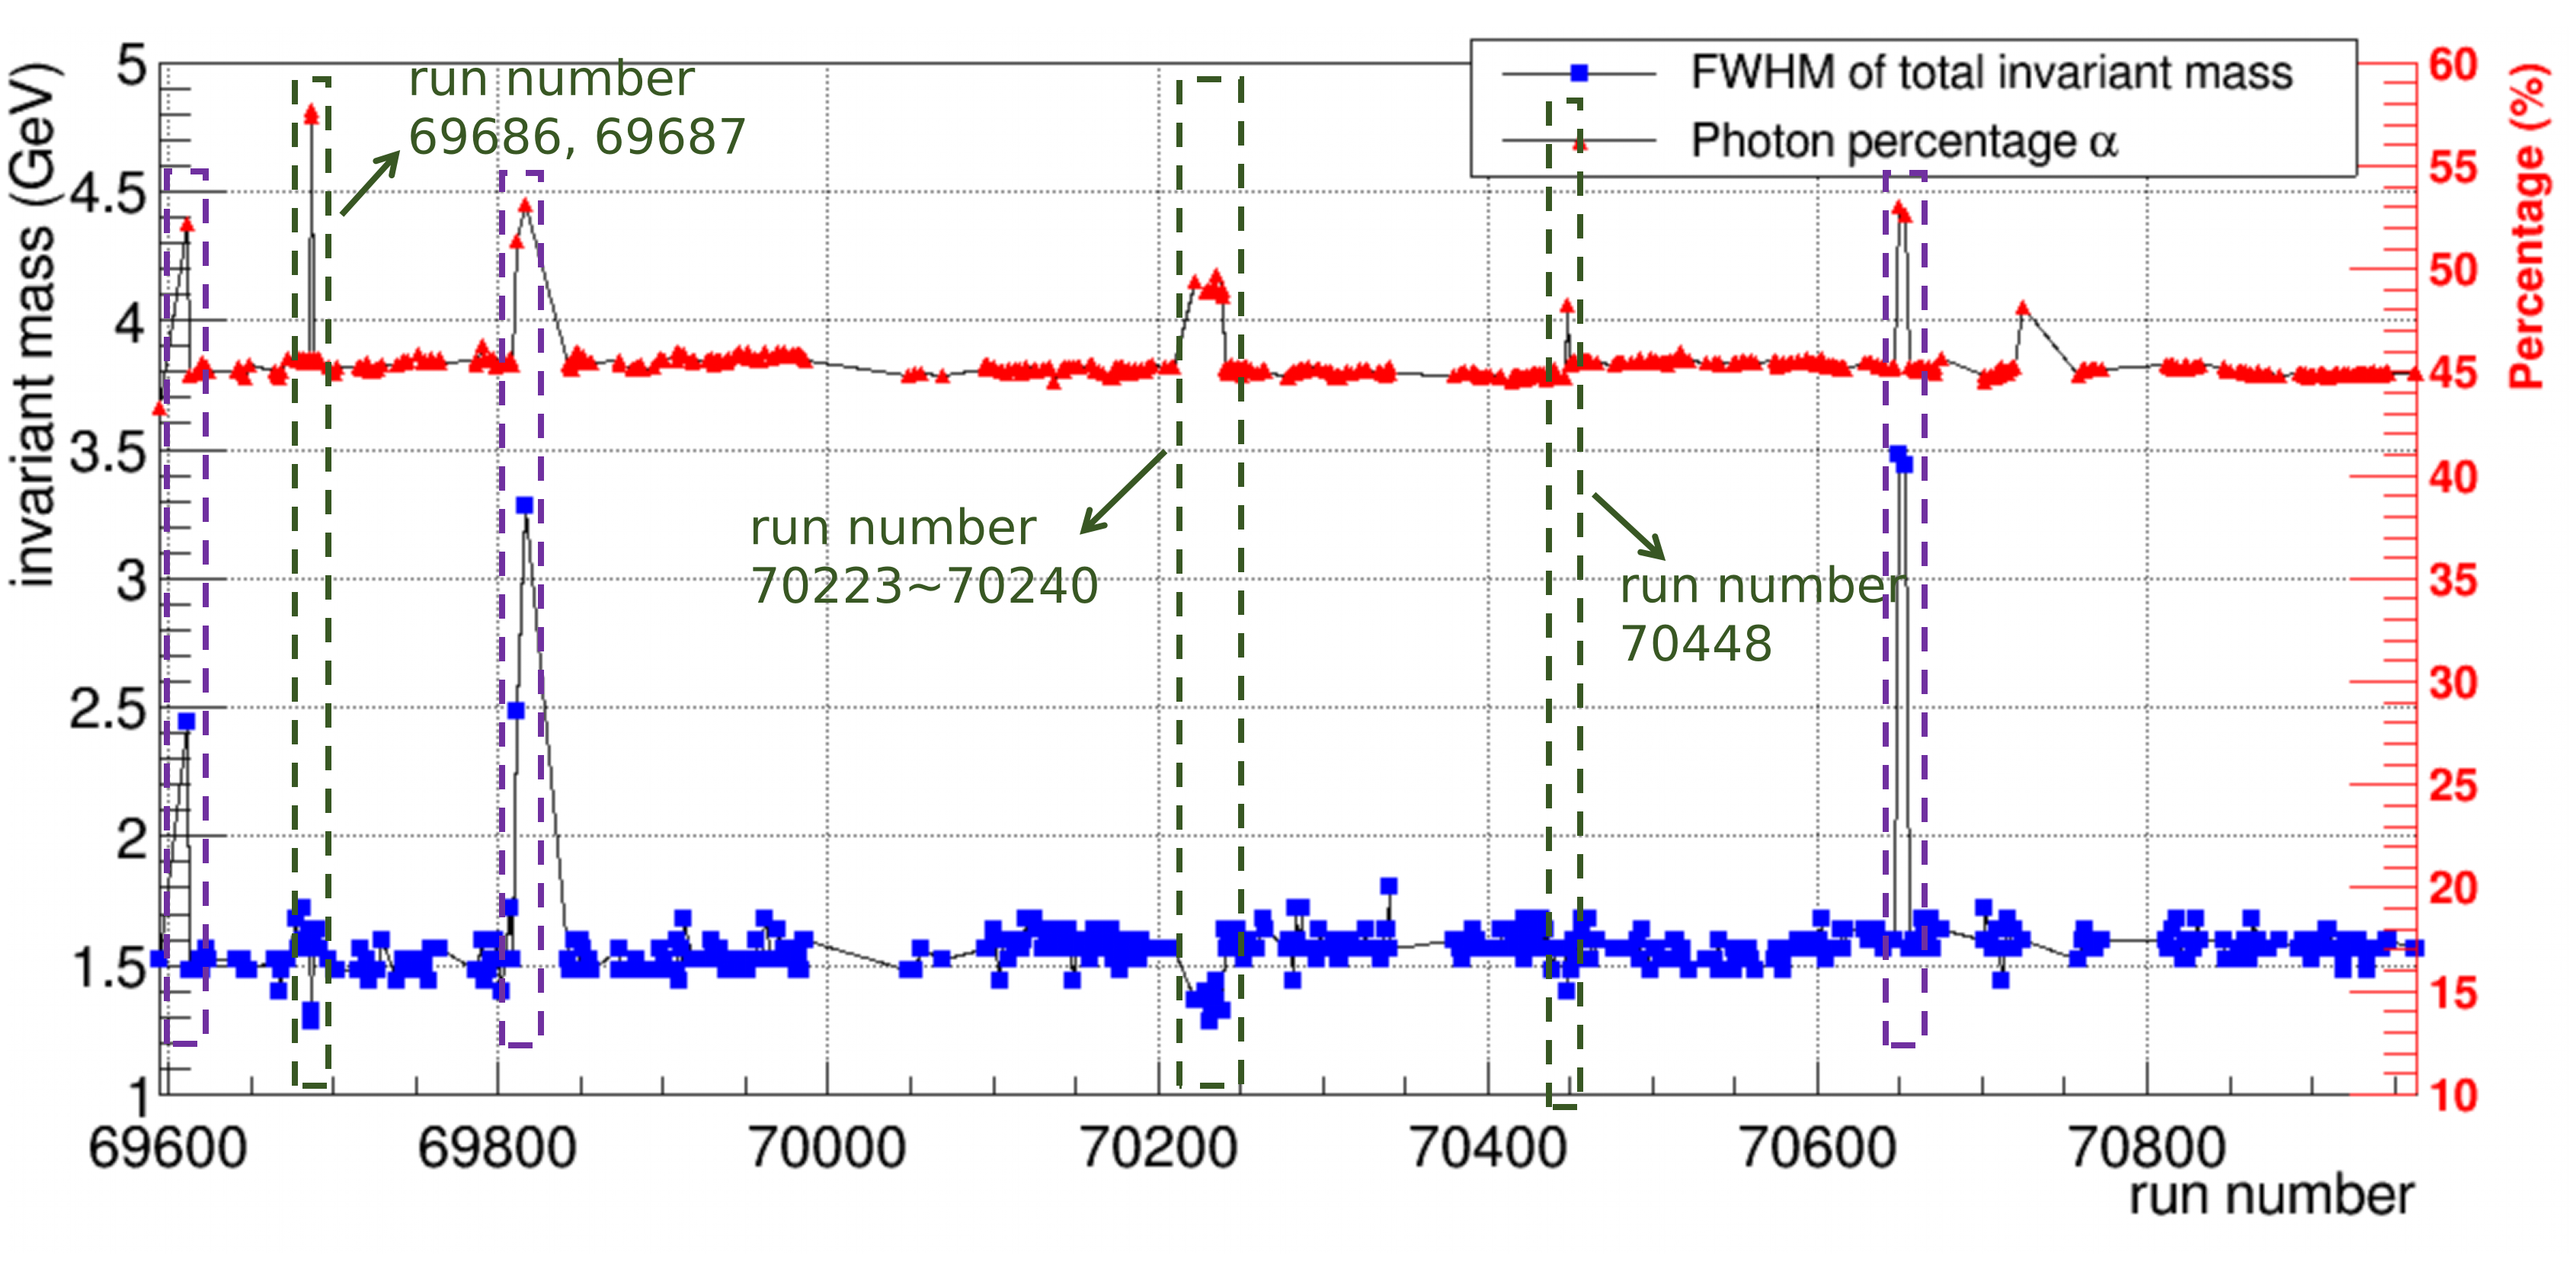
\includegraphics[width=\textwidth]{Total_mass_ECAL}
	\caption{Comparison between the FWHM value of total invariant mass (blue) and the photon number percentage $\alpha$ of calorimeters (red). For the normal runs, $\alpha$, the percentage of ECAL1, is about $45\%$. Apart from the positively correlated region (purple boxes) which has already existed in recoil proton width, there are three more negatively correlated regions (green boxes): 69686$\sim$69687, 70223$\sim$70240 and 70448. Additionaly, the negative correlated regions only have a smaller deviation value than positive correlated regions.}
	\label{fig:Total_mass_ECAL}
	\vspace{1cm}
\end{figure*}

\begin{figure*}[!h]
	\centering
	\vspace{1cm}
	\begin{subfigure}{\textwidth}
		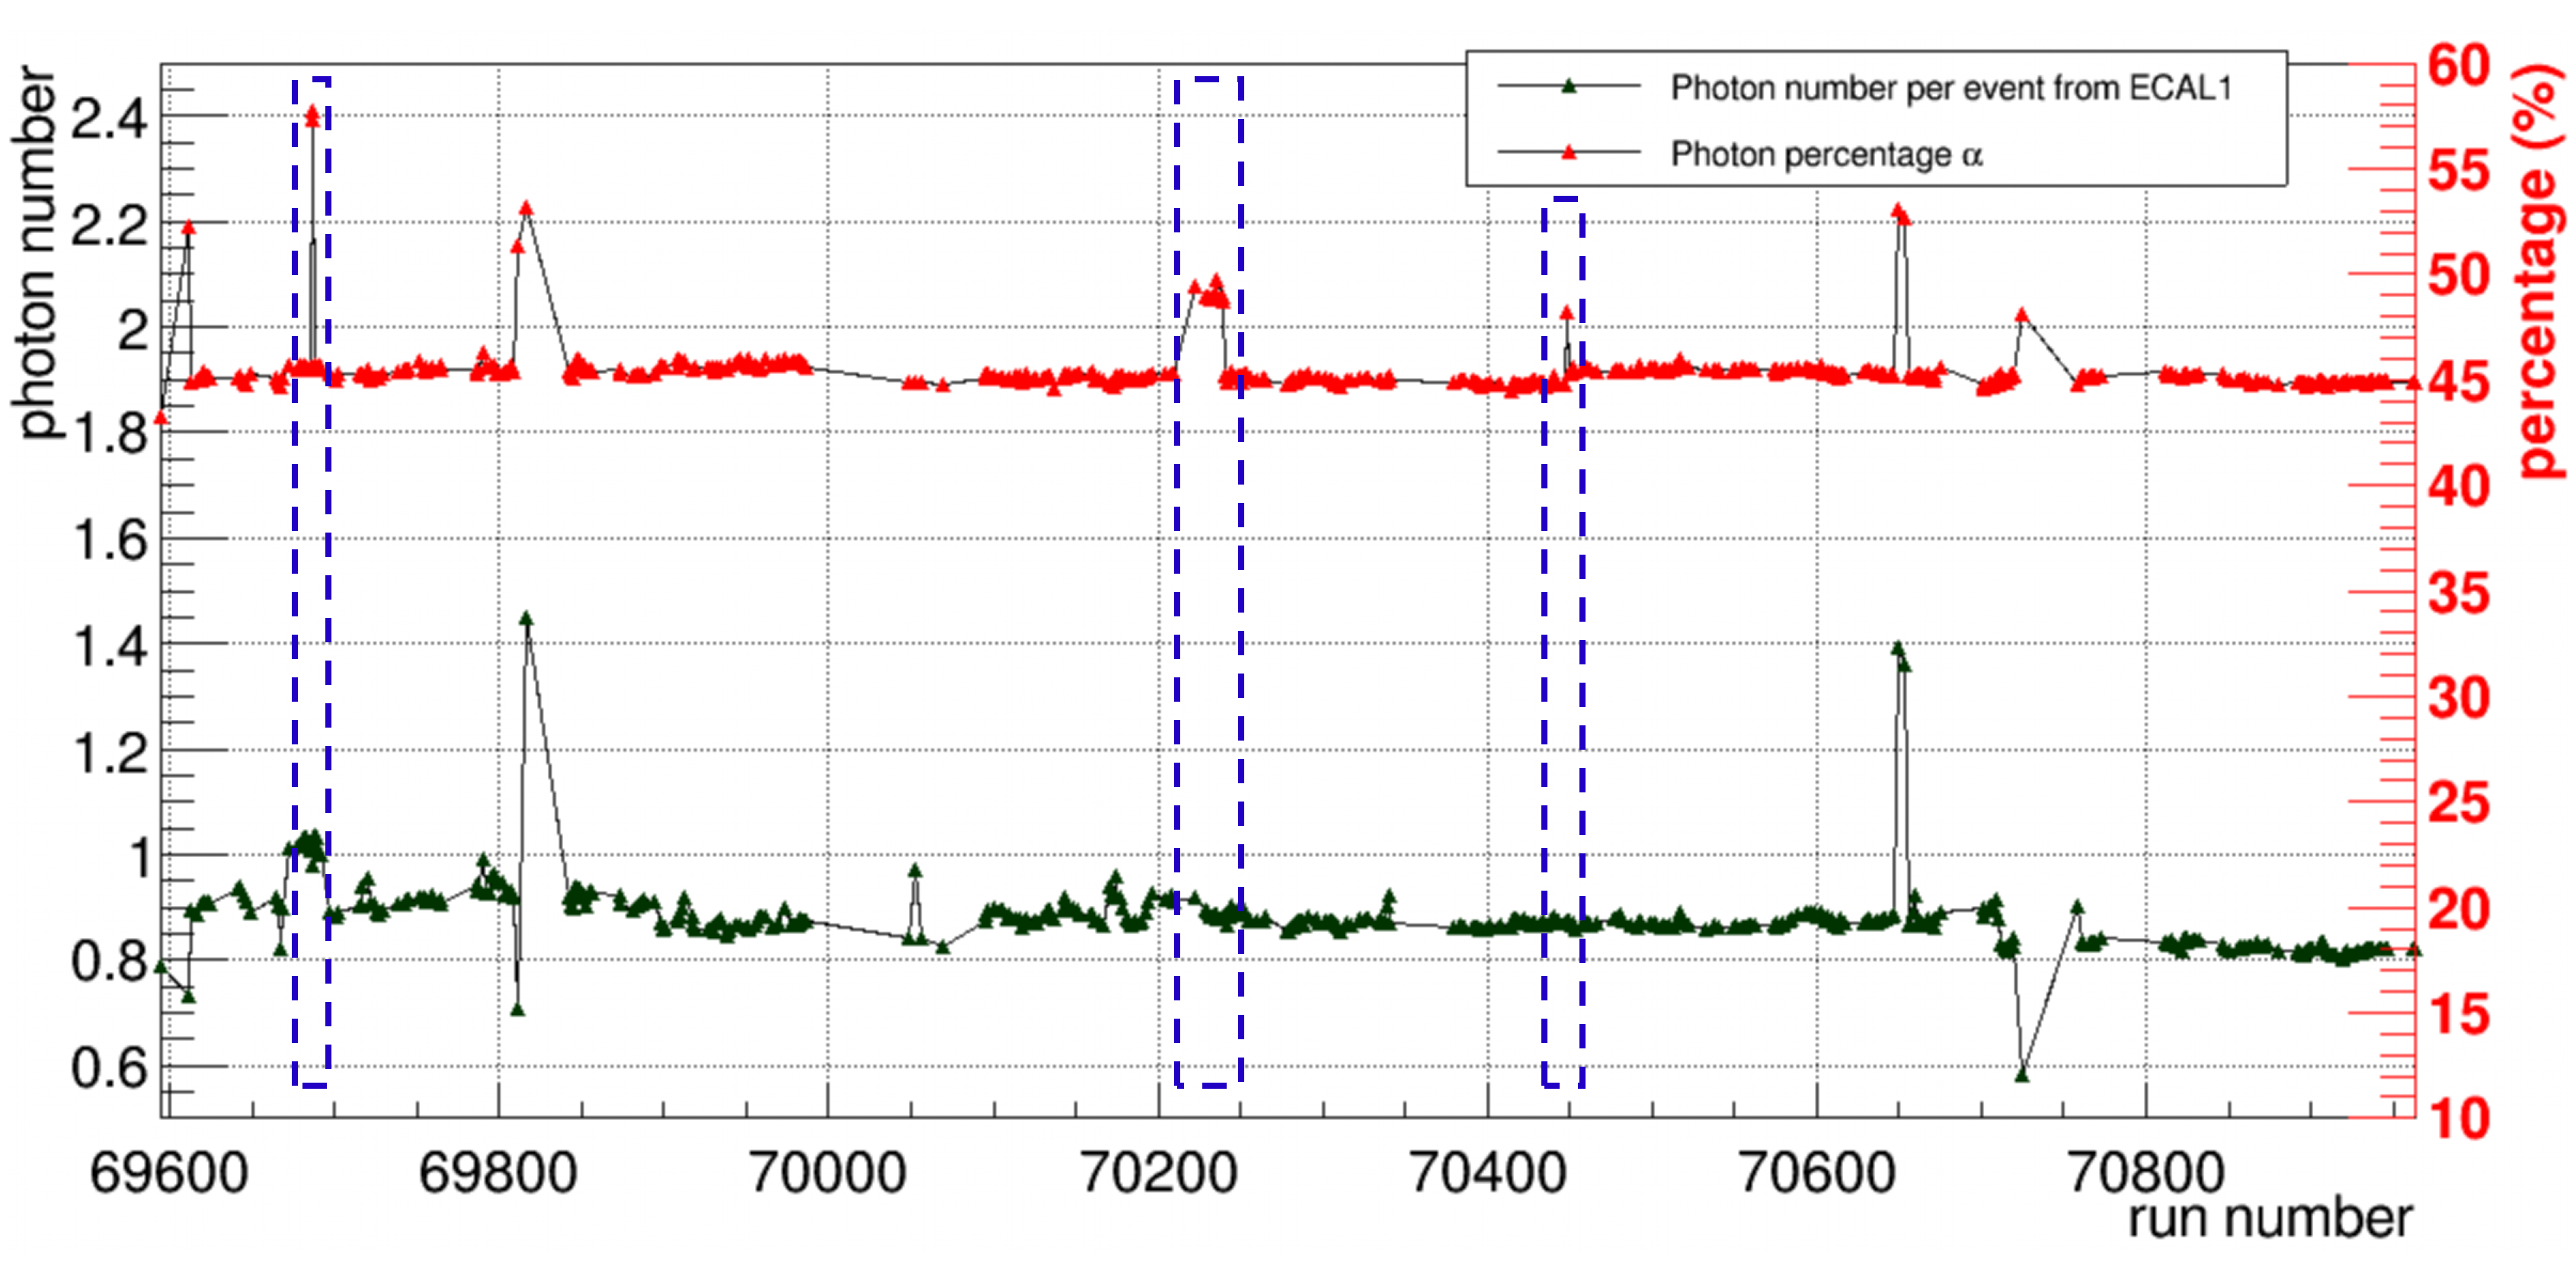
\includegraphics[width=\textwidth]{ECAL_per_ECAL1}
		\caption{ECAL1}
		\label{fig:ECAL_per_ECAL1}
		\vspace{1cm}
	\end{subfigure}
	\begin{subfigure}{\textwidth}
		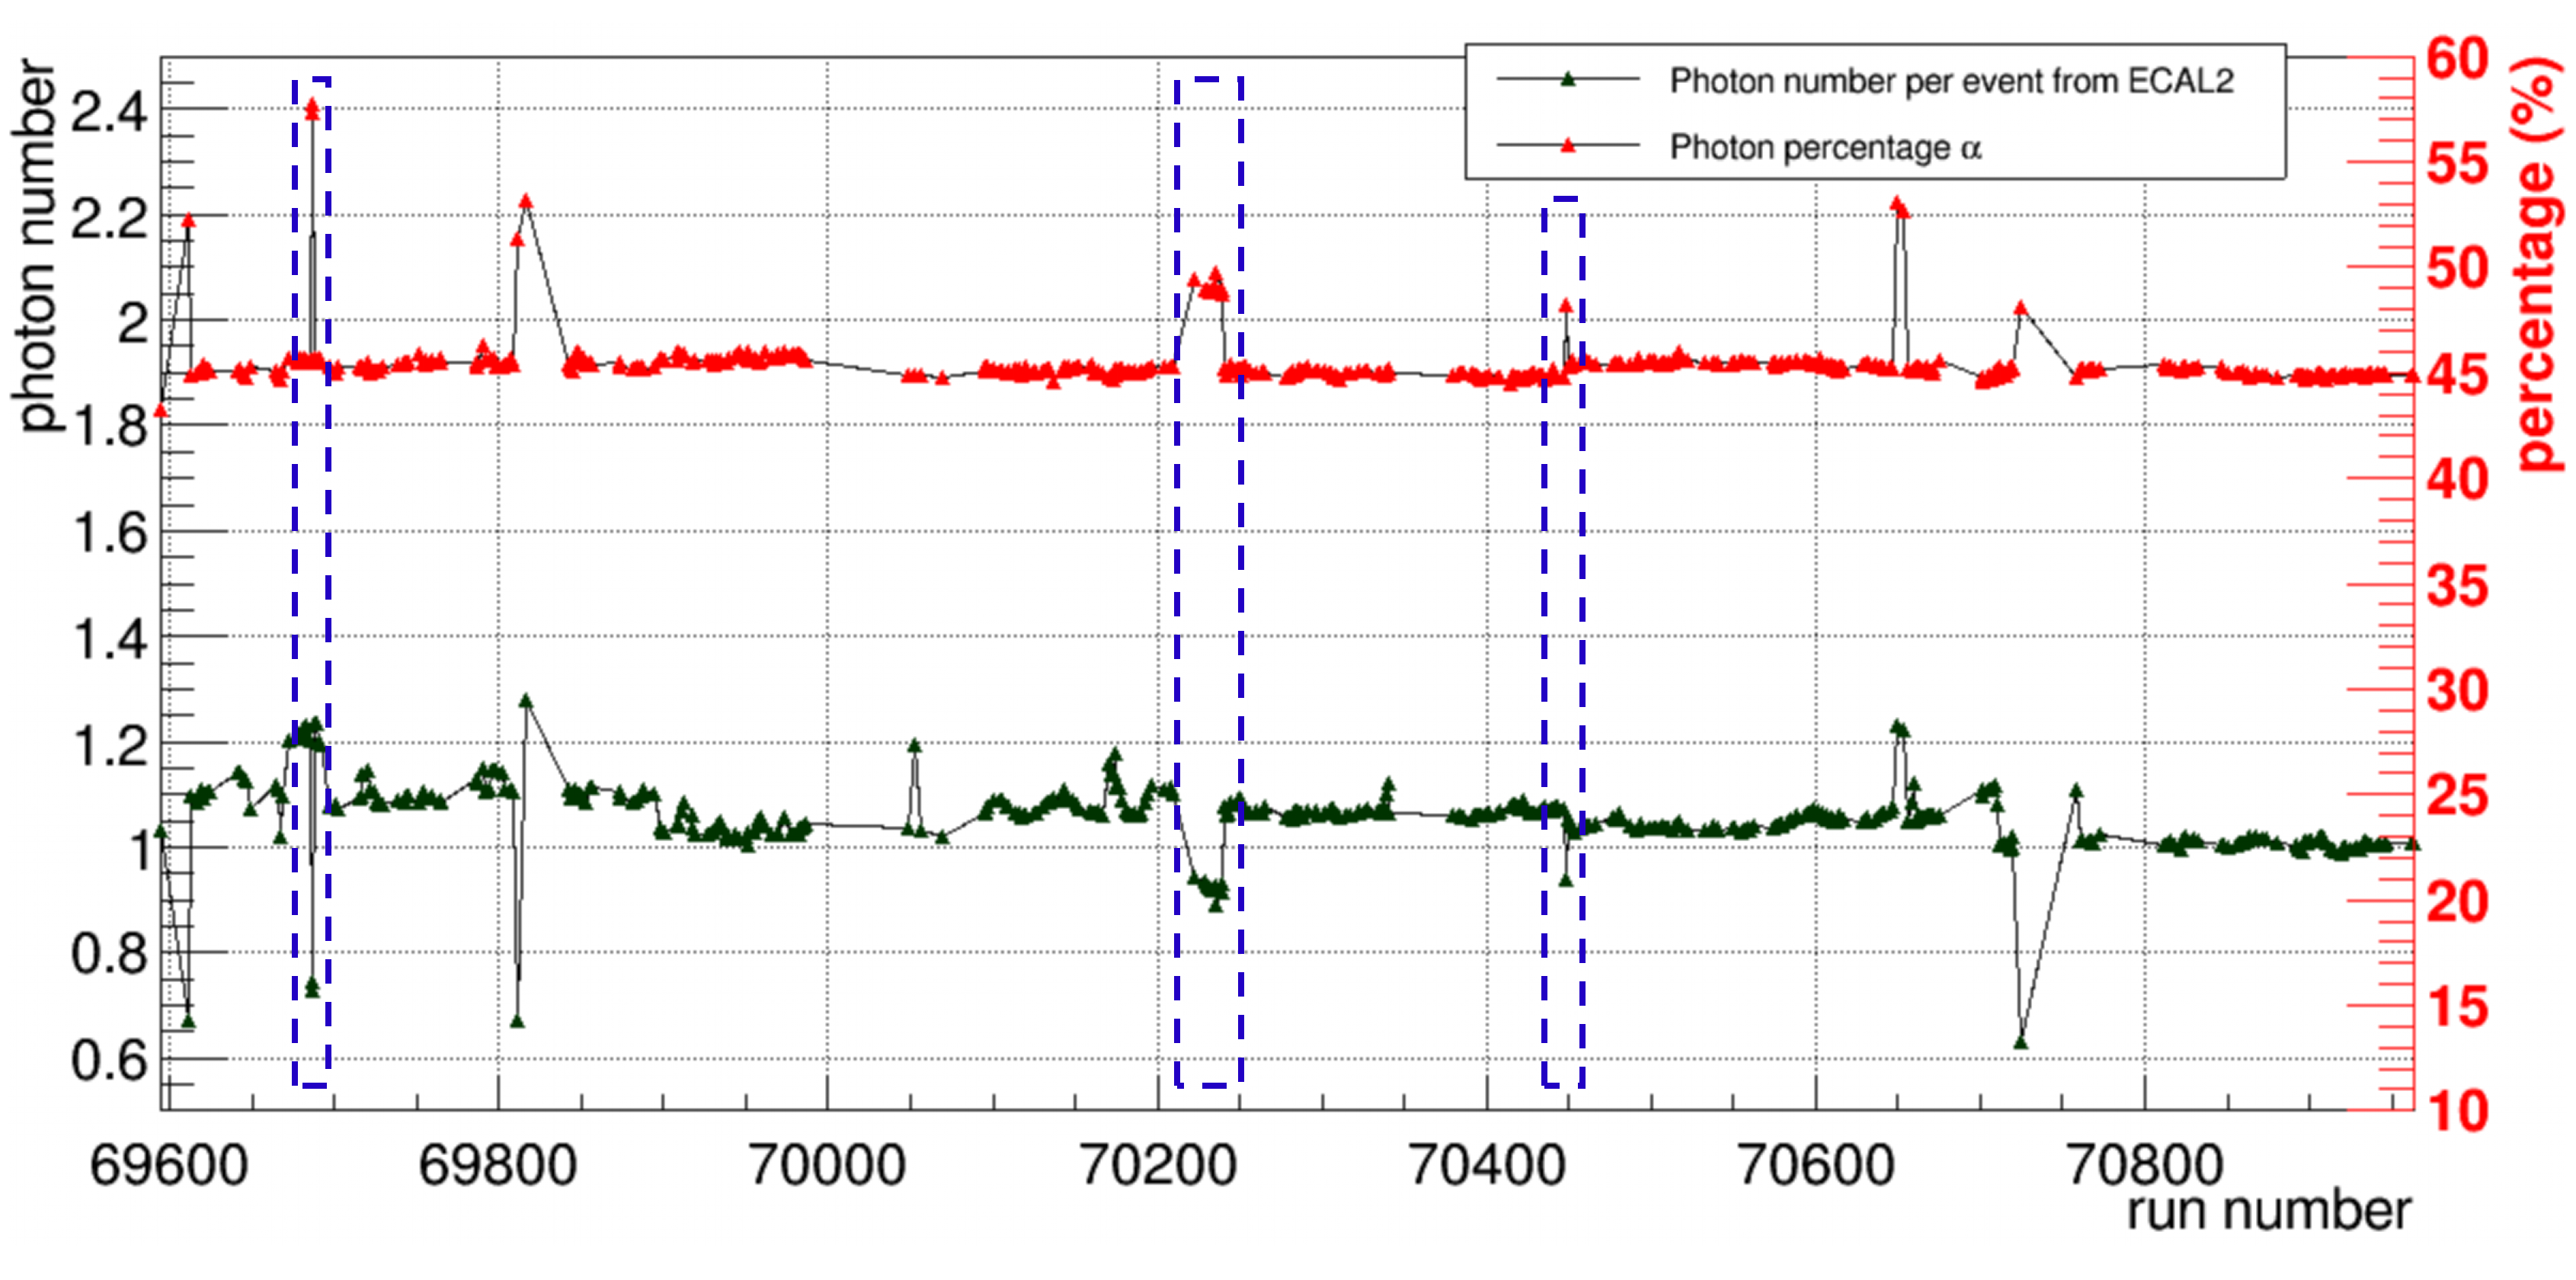
\includegraphics[width=\textwidth]{ECAL_per_ECAL2}
		\caption{ECAL2}
		\label{fig:ECAL_per_ECAL2}
	\end{subfigure}
	\caption{Detailed investigation of variation of $\alpha$, the photon number percentage of ECAL1. Averaged photon numbers for both two ECALs are calculated by dividing the total number of photon by the corresponding number of events in each run. Three negative correlated regions are shown by purple boxes. (a) comparison between the $\alpha$ (red) and photon number per event from ECAL1 (green). No abnormality appears in correlated regions for ECAL1. (b) comparison between the $\alpha$ (red) and photon number per event from ECAL2 (green). Declines of ECAL2 photon number are found in all negative correlated regions.}
	\label{fig:ECAL_per_ECAL}
	\vspace{1cm}
\end{figure*}

The second type of abnormality (run 70054) is shown in figure \ref{fig:Recoil_proton_double_peak}, where another peak occurs at about \SI{2.7}{\radian} to \SI{2.8}{\radian}. Theoretically speaking, the scattering angle $\theta$ cannot be larger than $\pi/2$ for the recoil proton since it cannot scatter backwards after being hit by a $\pi^-$. In reality, the reconstruction of the out-going particle tracks causes an uncertainty of primary vertex position and RPD reconstruction about recoil proton is also not very precise. Therefore, scattering angle $\theta$ has errors. This is the reason why even for a normal run, small amount of events contains the protons with recoiled at angles slightly bigger than $\pi/2$. For run 70054\footnote[2]{The abnormal run 70054 is ruled out for the following analysis} (shown in figure \ref{fig:Recoil_proton_double_peak}), there are even some recoil protons with recoil angles reaching to $\SI{2.7}{\radian}$. One of explanations of this phenomenon is a trigger defect. Due to this, primary vertex, which is used for calculating the recoil angle, is not in the same event of the corresponding recontructed recoil proton position. Therefore, the runs with such abnormality should be ruled out during analysis.






\section{Correlation and results}
As has been discussed in last section, different characteristic parameters are investigated throughout the whole runs. Except few cases such as long period of spill (see figure \ref{fig:EveN_spill_abnormal}) or double peaks from recoil proton (see figure \ref{fig:Recoil_proton_double_peak}), most of the abnormalities can be depicted by FWHM value of total invariant mass distribution (shown in figure \ref{fig:Total_mass_FWHM}). To decipher the cause behind all these phenomenon, correlations between the abnormalities of different parameters are inquired.
\subsection{Correlation of abnormalities}
The most two obvious parameters that can be correlated to the abnormality of total invariant mass distribution should be recoil proton and photon number captured by both ECALS.
\subsubsection{Correlation with recoil proton}
The angular distribution of recoil proton is directly related to the scattering process. If spectrum and constitution of incoming particle beam are same for each run, the mass of unknown intermediate state $X$ can be reflected by the recoil proton due to four-momentum conservation. As is shown in subsection \ref{subsec:recoil_proton}, the width at lower half of angular distribution could be really large for abnormal runs. To establish the correlation, the value of width for recoil proton can plotted with the value of FWHM of invariant mass distribution for each run (see figure \ref{fig:Total_mass_recoil_proton}). At first sight, strong correlations appear for the run number 69816, 70650, 70654. When there is an increase on FWHM value, there is also an increase on the width from recoil proton. On the other hand, there are also some abnormal runs which are not correlated, such as run number 69811 and range 70223 $\sim$ 70240.
\begin{figure*}[!h]
	\centering
	\vspace{2cm}
	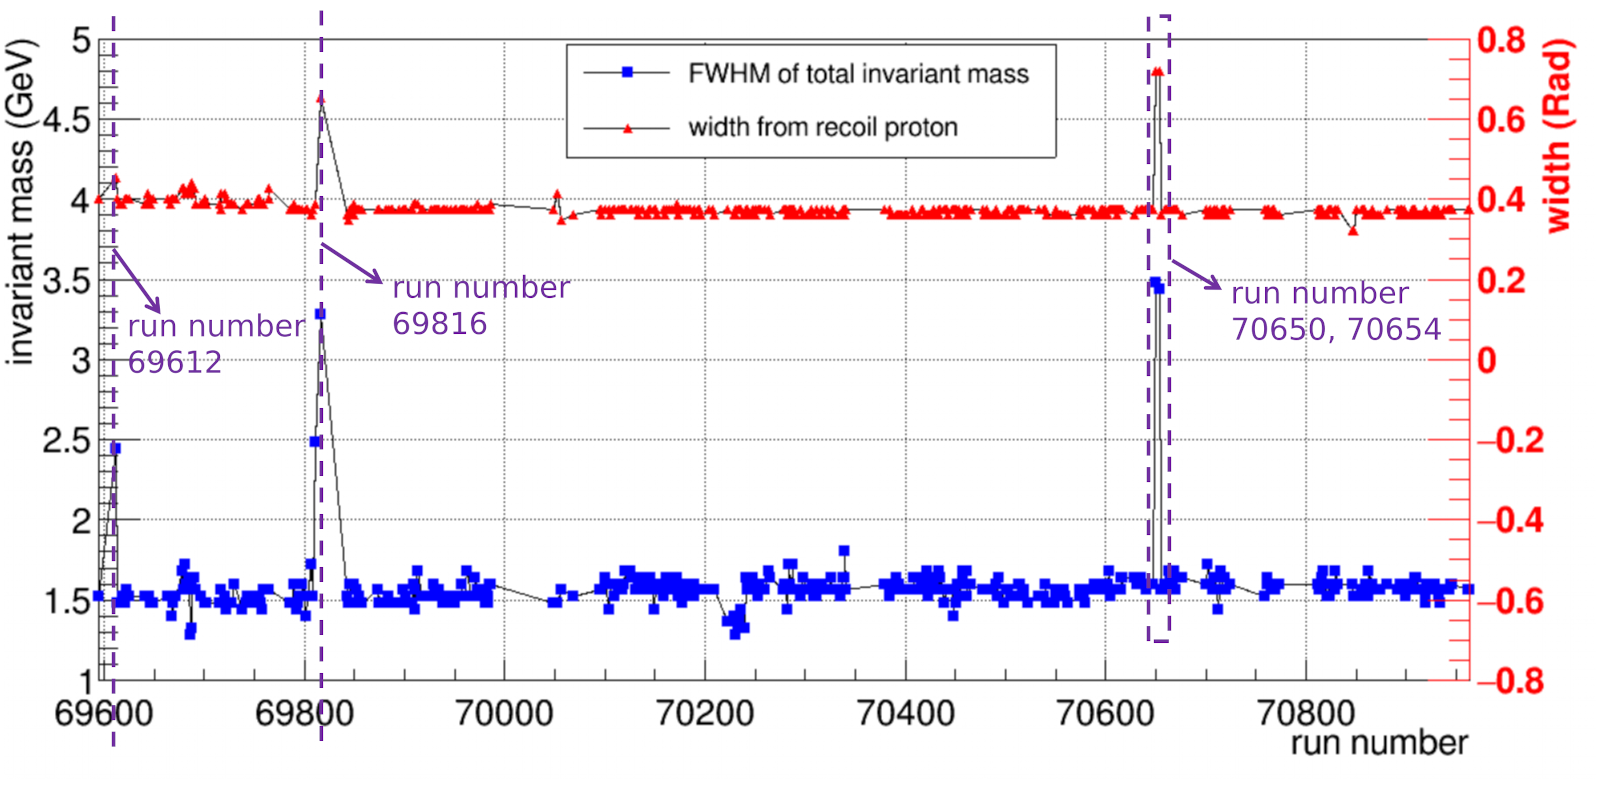
\includegraphics[width=\textwidth]{Total_mass_recoil_proton}
	\caption{Histogram of invariant total mass distribution. The colors inside the histogram represent number of events corresponding to the run number and invariant mass. To better compare and conceive the structure of distribution between runs visually, the maximal value of each distribution is normalized to 1000. In the red dashed rectangles, it can be seen that the red strokes are much longer than the normal runs.}
	\label{fig:Total_mass_recoil_proton}
	\vspace{2 cm}
	
	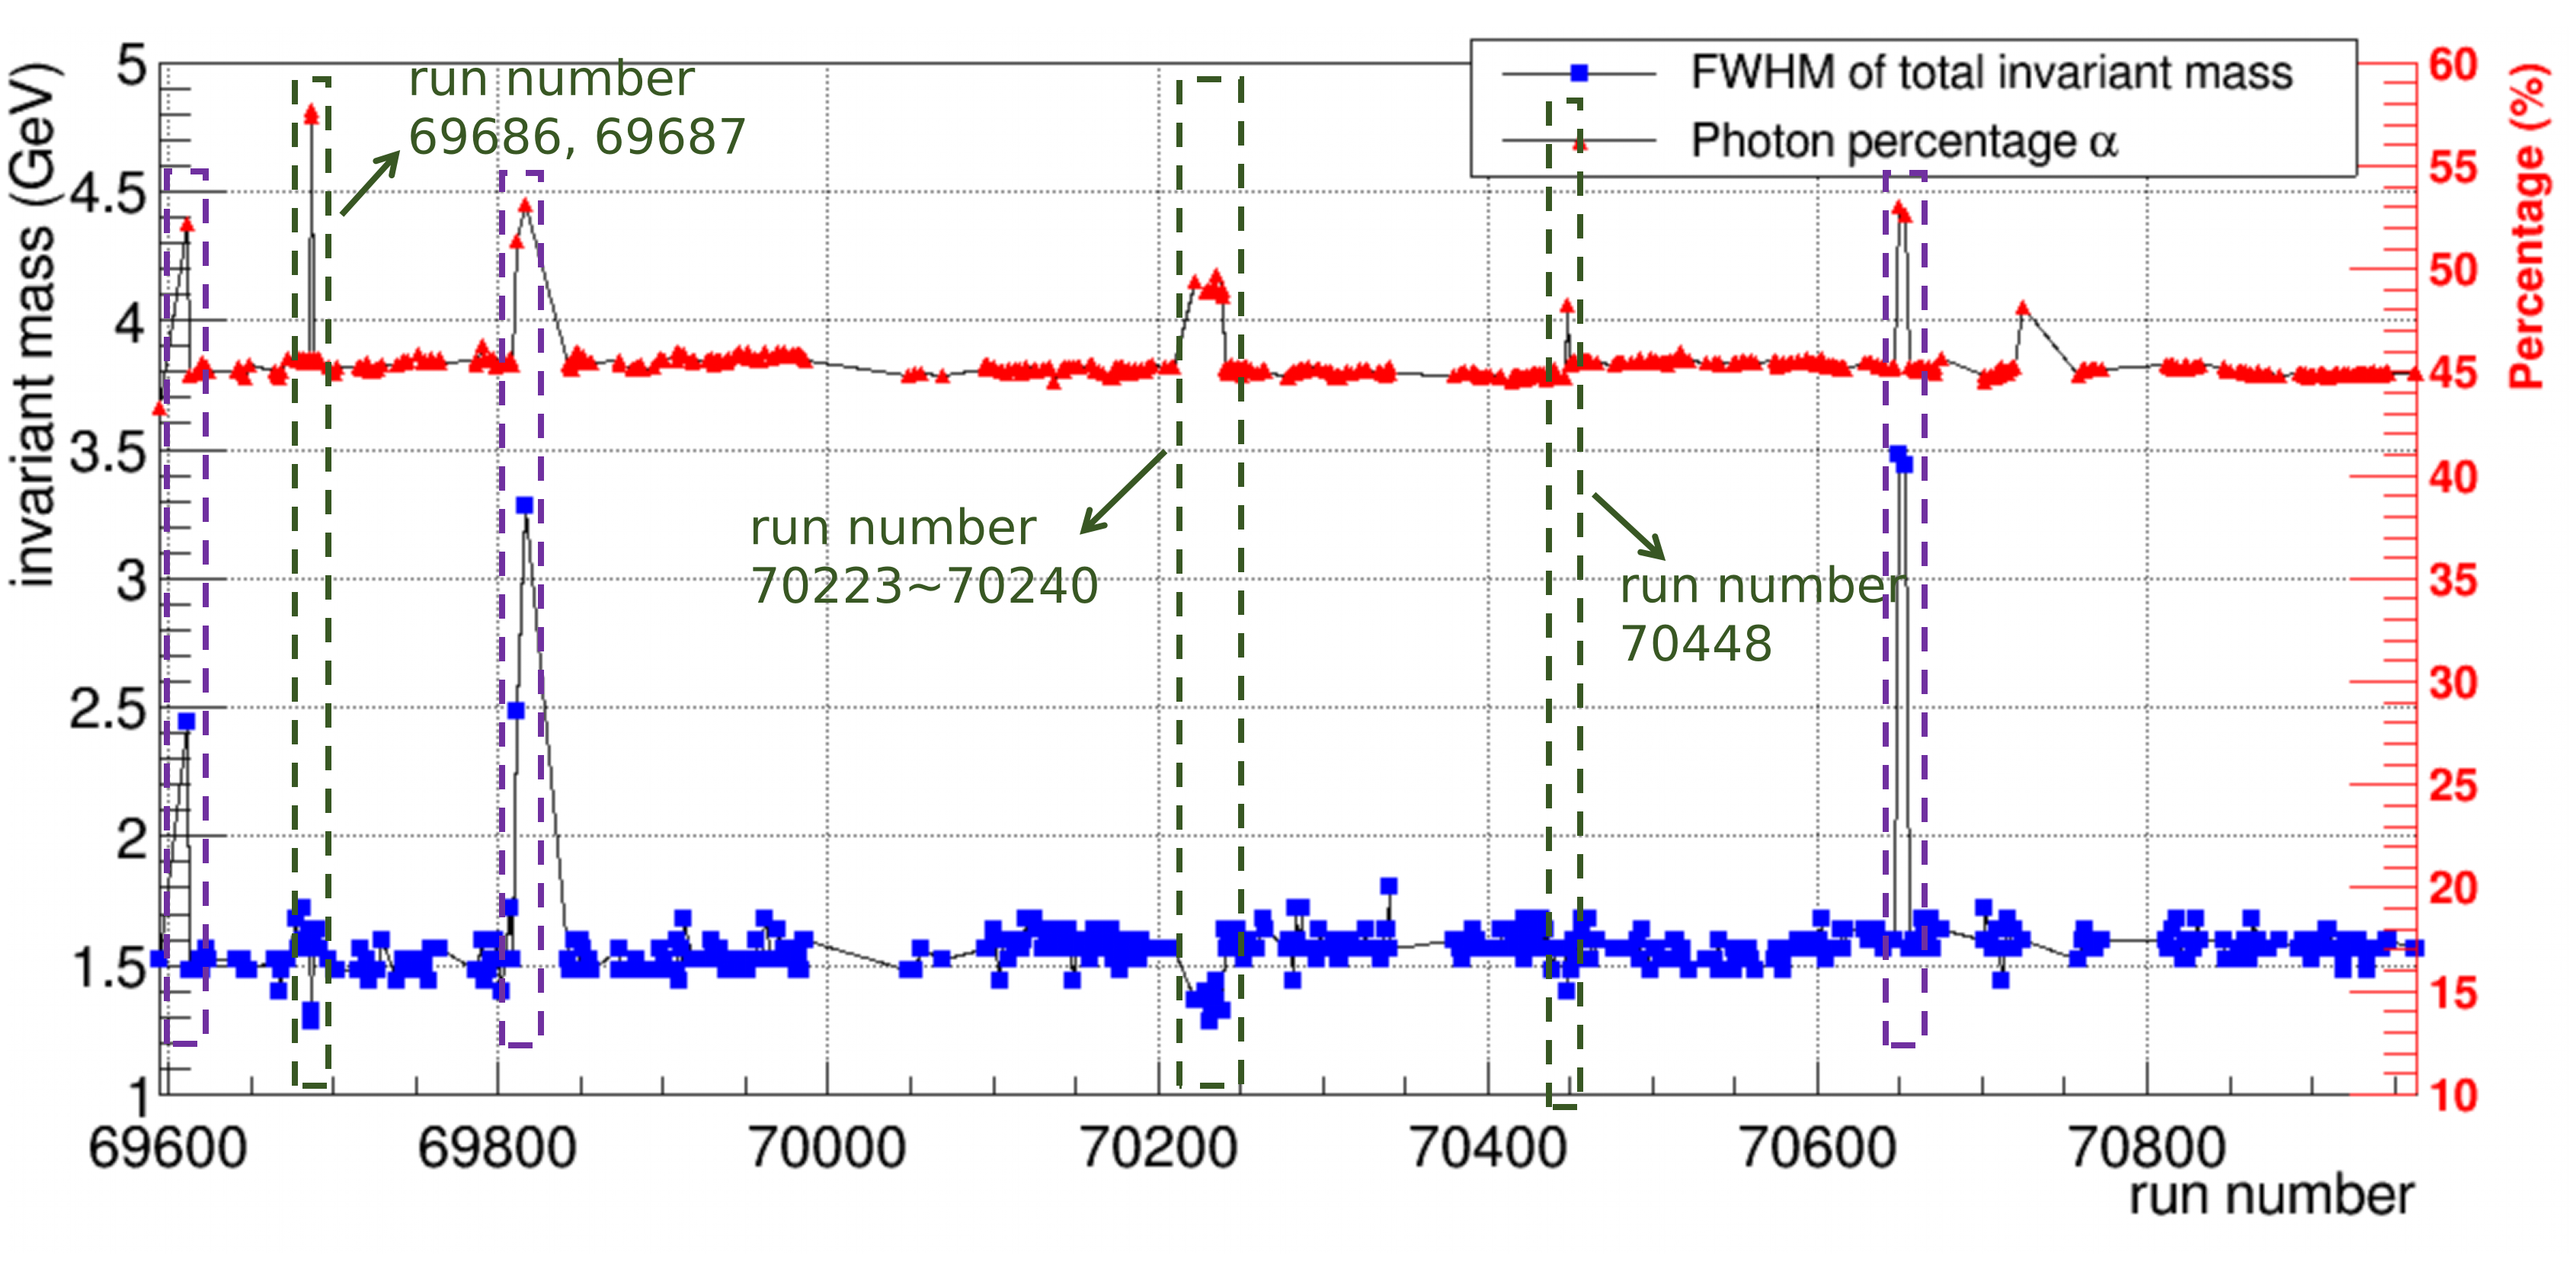
\includegraphics[width=\textwidth]{Total_mass_ECAL}
	\caption{Value of full width at half maximum of total invariant distribution for each run. Typical value of FWHM for normal run is around \SI{1.5}{\giga\electronvolt}.There are several outliners that have much bigger FWHM value than the general one. Also there is a range of runs 70223 $\sim$ 70240 that have slight smaller value of FWHM. }
	\label{fig:Total_mass_ECAL}
	\vspace{3cm}
\end{figure*}
\subsubsection{Correlation with ECALs}
Comparing abnormal runs in figure \ref{fig:Total_mass_FWHM} and figure \ref{fig:Three_pion_mass_Graph}, one can easily notice that most of abnormal runs in total invariant mass distribution fail to show abnormality in invariant mass distribution of three pions.
\subsection{Summary of abnormal runs}
\begin{table}[!h]
	\begin{tabular}{|p{0.1\textwidth}|p{0.15\textwidth}|p{0.2\textwidth}|}
		\hline
		RunNumber        & Abnormality                                      & Log book/comments                 \\ \hline \hline
		70195             & Disorder of spill time                                    & Good                              \\ \hline \hline
		69811             & Three pion mass                                           & Magnets were ramped up during run \\ \hline \hline
		70054             & Double peaks for recoiled proton                          & Errors appeared for SrcID         \\ \hline \hline
		69612             & \multirow{4}{0.15\textwidth}{Recoiled proton angular distribution}     & N/A                               \\ \cline{1-1} \cline{3-3} 
		69816             &                                                           & No sandwich veto                  \\ \cline{1-1} \cline{3-3} 
		70650             &                                                           & Special run to test sandwich veto \\ \cline{1-1} \cline{3-3} 
		70654             &                                                           & No sandwich veto                  \\ \hline \hline
		\parbox[c]{\hsize} {69696}             & \multirow{4}{0.15\textwidth}{Decrease of number of photons from ECAL2} & Detector test                     \\ \cline{1-1} \cline{3-3} 
		69687             &                                                           & Light trigger problems            \\ \cline{1-1} \cline{3-3} 
		70223 $\sim$70240 &                                                           & High voltage trip on ECAL2        \\ \cline{1-1} \cline{3-3} 
		70448             &                                                           & Low intensity beam                \\ \hline
	\end{tabular}
\end{table}
\section{Conclusion}
In this project, to analysis the instability of different runs from COMPASS experiment, different parameters are extracted or calculated for each run. Among characteristic parameters such as the total number of events or invariant mass of three pions, the total invariant mass of out-going particles prove to be the most indicative parameters. Its correlation with ECAL1 photon number percentage ($\alpha$) encompasses most of abnormal runs found during stability test. The positive correlated regions also indicate the abnormality in angular distribution of recoil proton whereas negative correlated regions are related to the decline of ECAL2 averaged photon number per event. By checking out the logbook of experiment, some abnormality could be well explained such as the malfunctions of sandwich veto or solenoid magnet.

% BIBLIOGRAPHY
\bibliographystyle{plain}
\clearpage
\bibliography{references}

%Appendix
%\cleardoublepage

%\input{chapters/Appendix}
\end{document}


